\chapter{Emotion Machine Cognitive Architecture}
\label{chapter:emotion_machine_cognitive_architecture}

The SALS cognitive architecture is inspired by the bottom four layers
of the {\emph{Emotion Machine}} theory of human commonsense thinking
described by \cite{minsky:2006}.  SALS includes architectural
primitives for defining different types of reflective AIs.  The most
basic component of the SALS architecture is an object called a
{\emph{resource}}.  In general, a resource is any compiled procedure
that can be executed by activating the resource.  A resource is said
to be {\emph{activated}} if it is currently executing.  A resource may
be activated as an action in a plan.  If a resource is currently
executing, a {\emph{duplicate activation failure}} results from an
attempted additional activation of the resource.  If a resource is not
currently activated, a resource may be {\emph{suppressed}}, which is a
logical internal state of the resource that causes any attempts to
activate the resource to result in a {\emph{suppressed activation
    failure}}.  Resources are usually assigned simple functions that
do not do complicated or intelligent reasoning tasks themselves, but
instead, resources are generally designed so that they perform
primitive activities that can be combined in various ways to perform
various resultingly complex tasks.  For example, the simplest
resources in the SALS AI that interact directly with the physical
simulation do simple tasks like: ``{\tt{start moving left}},''
``{\tt{start moving right}},'' ``{\tt{stop moving}},''
``{\tt{reach}},'' and ``{\tt{grab}}.''  Resources may be activated or
suppressed by plans in the layer above those resources.  If a resource
is suppressed and activated at the same time, this results in an
activation failure that causes a plan to stop executing, so that it
may be reflectively debugged at a higher layer.  Some resources in
SALS are referred to as {\emph{vital resources}} because they are
activated when the AI is initially created and they never complete
execution.  For example, one vital resource monitors any changes to a
visual knowledge base and attempts to create a stable physical model
of the world from these changes.  Vital resources are usually used for
processing streams of reflective trace events that monitor and learn
from the effects of other executing resources.

Resources are grouped into collections called {\emph{agencies}}.
Agencies tend to be used for combining resources that are used for
accomplishing similar types of goals.  For example, the low-level
resources that control the physical simulation are referred to as a
{\emph{physical agency}}.  Resources that can be activated and used
for solving problems are usually grouped into agencies that separate
them from the vital resources.  For example, the vital resources that
process low-level visual knowledge trace events are separated into a
{\emph{sensory agency}}.

Agencies are further grouped into collections called {\emph{layers}}.
The SALS AI consists of five layers of reflective control.  These
layers are:
\begin{samepage}
  \begin{packed_enumerate}
  \item{{\emph{The Built-In Reactive Layer}}}
  \item{{\emph{The Learned Reactive Layer}}}
  \item{{\emph{The Deliberative Layer}}}
  \item{{\emph{The Reflective Layer}}}
  \item{{\emph{The Super-Reflective Layer}}}
  \end{packed_enumerate}
\end{samepage}
{\mbox{\autoref{figure:five_layers_overview}}} shows an overview of
the five layers of the reflective AI.
\begin{figure}
\centering
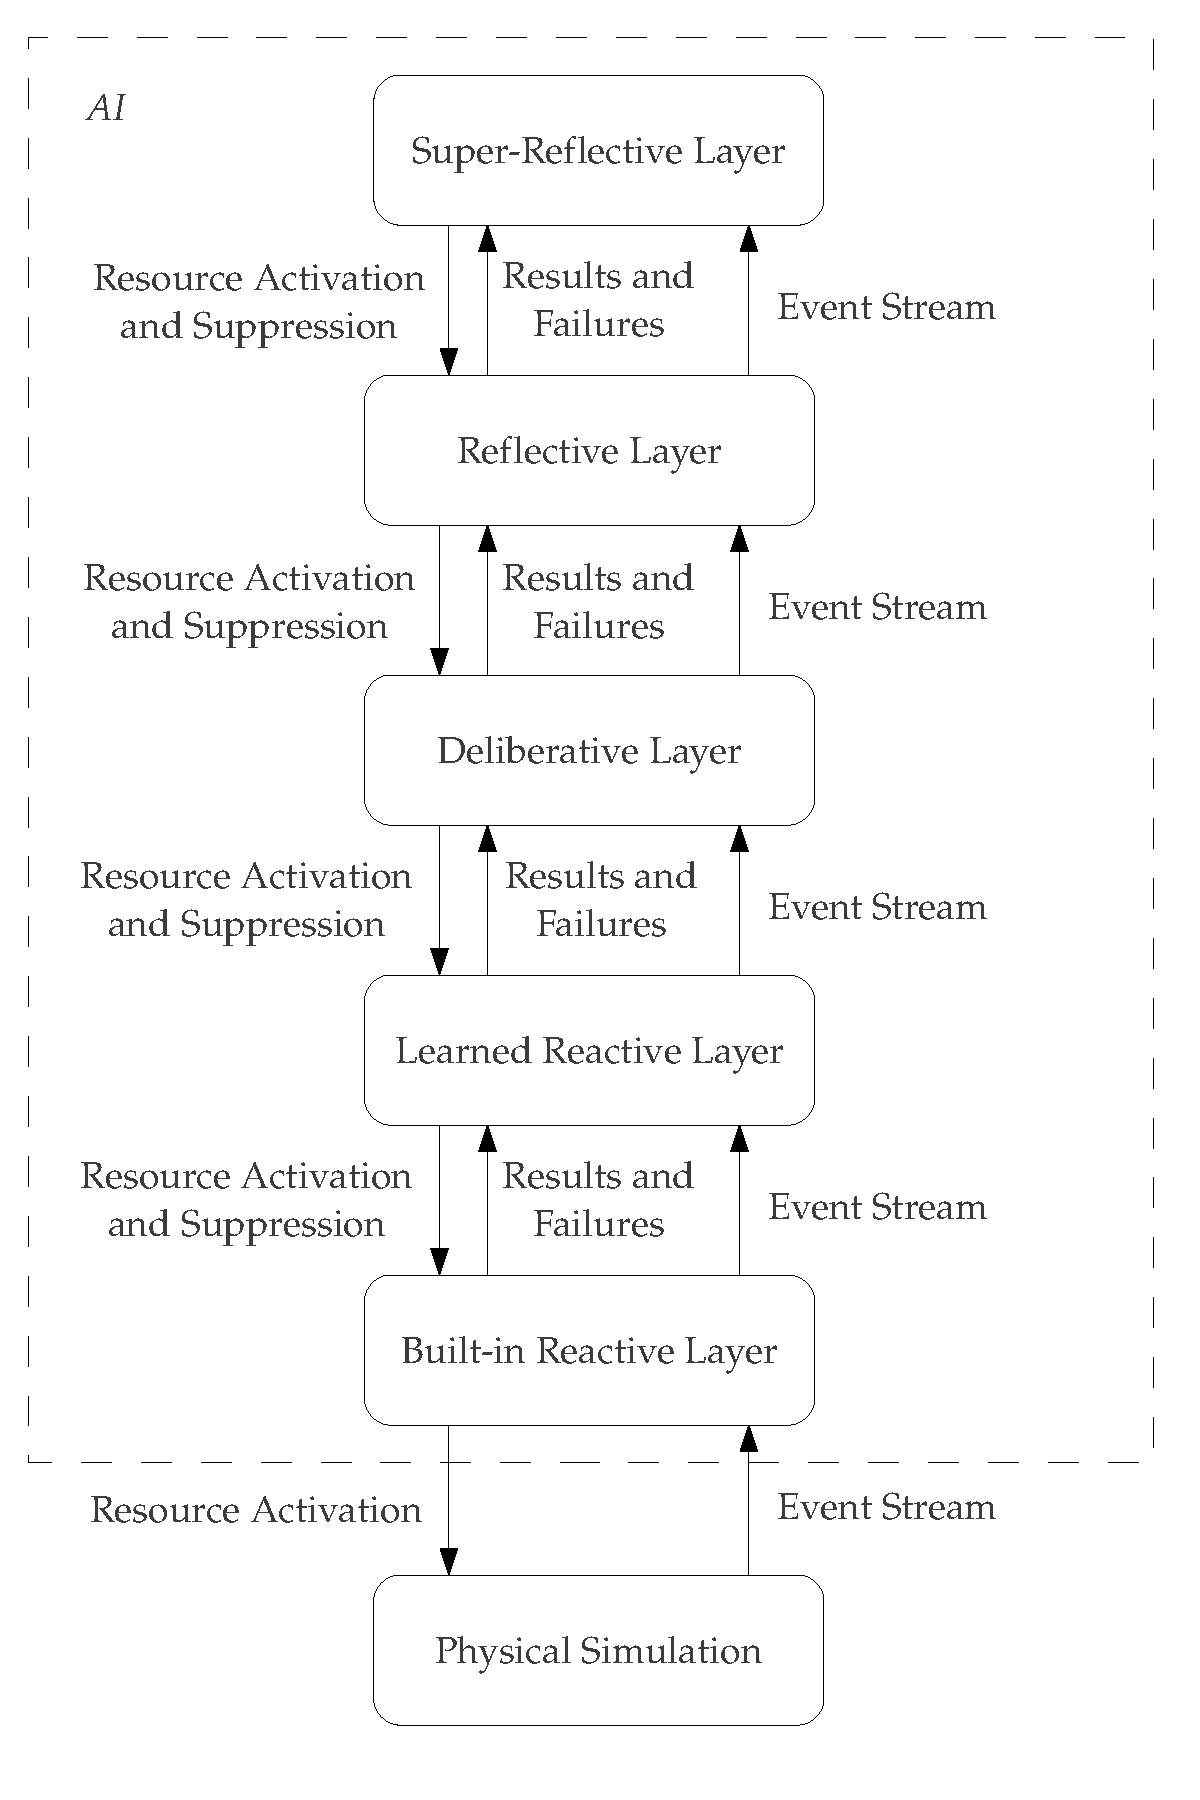
\includegraphics[width=10cm]{gfx/five_layers_overview}
\caption[The five layers of the AI in relation to the physical
  simulation.]{The five layers of the AI in relation to the physical
  simulation.}
\label{figure:five_layers_overview}
\end{figure}
The layers of the AI form cascaded control loops, where each layer
controls the layer below.  One would expect that in a real human there
are cases where lower layers activate and suppress upper layers, such
as hunger suppressing rational deliberation.  In SALS, this is
implemented as a reflective process that executes a deliberative plan
that periodically checks a specific negative physical goal state
exists and fails if it does, which would cause the reflective process
to suppress the appropriate deliberative resources.

\section{The Physical Simulation}

The physical simulation that is used to demonstrate the SALS AI,
depicted in
{\autoref{figure:introduction_example_problem_domain__duplicate_1}},
is similar to the {\emph{Blocks World}} planning domain
\begin{wrapfigure}{r}{6.125cm}
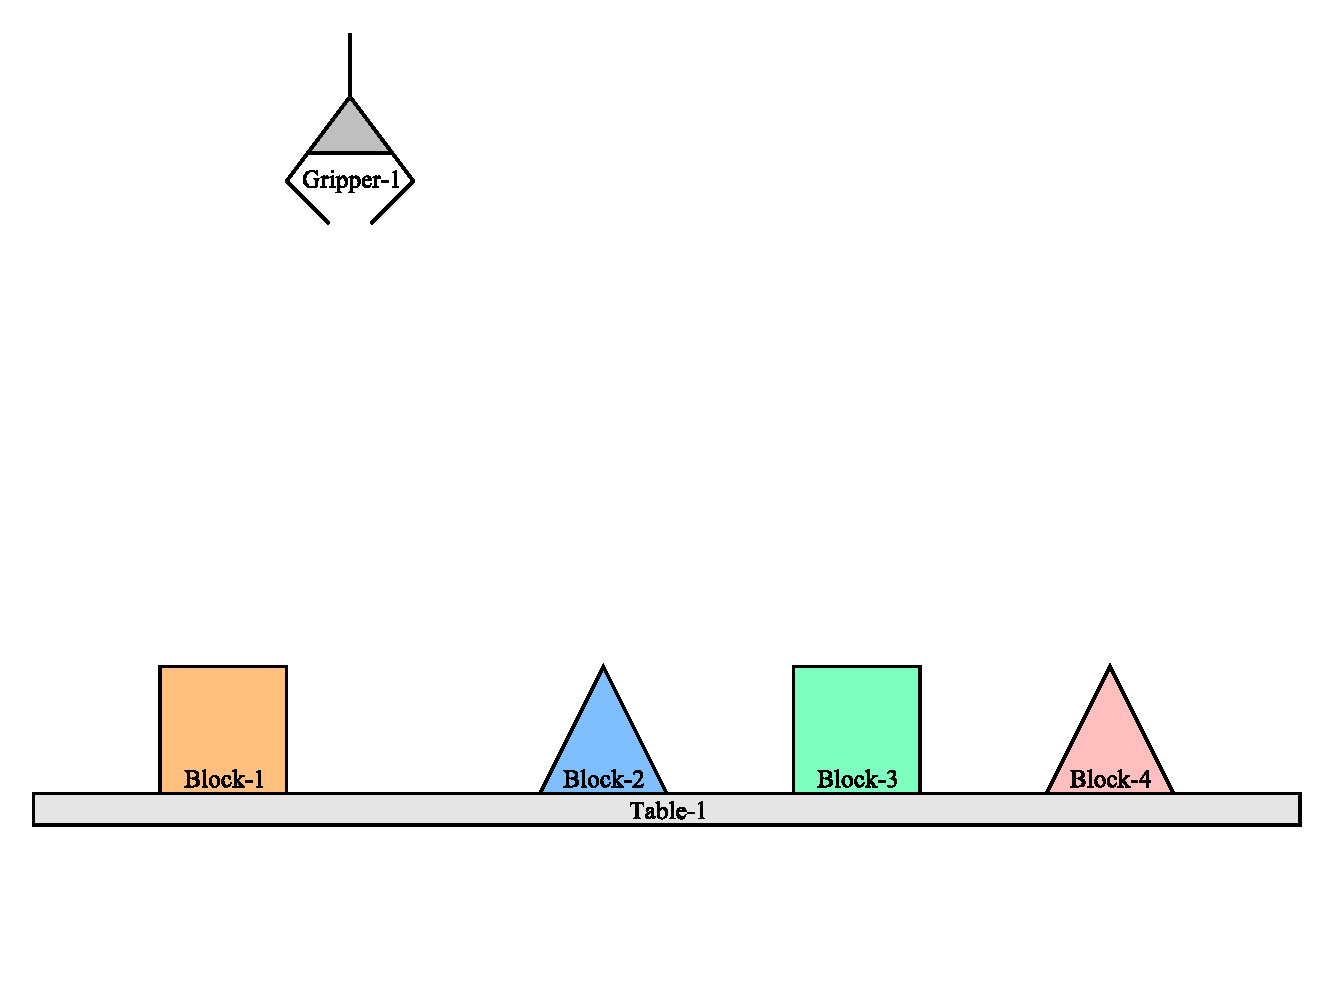
\includegraphics[width=6cm]{gfx/blocks_world_large-01}
  \caption[An example {\emph{Blocks World}} problem domain.]{An
    example {\emph{Blocks World}} problem domain, duplicated from
    {\mbox{\autoref{figure:introduction_example_problem_domain}}}.}
  \label{figure:introduction_example_problem_domain__duplicate_1}
\end{wrapfigure}
{\cite[]{winograd:1970}}.  The physical simulation is a 2-dimensional,
deterministic, rigid-body physical simulation based upon a
floating-point implementation of Newtonian physics ($F=ma$).  The
simulation is stepped with a time step of $0.1$ seconds.  The gripper
can be controlled by the SALS AI to move left or right at one of two
different speeds, fast ($1\text{ m}/\text{s}$) or slow ($0.25\text{
  m}/\text{s}$).  The simulation is meant to be a model of a
continuous-time domain, rather than the logical propositional type of
domain that is often used in other Blocks World simulations.  The
dexterous manipulation problem of the gripper picking up a block is
simplified by simply allowing the gripper to magically grab a block
when it touches the top of the block.  When a square block is dropped
on top of a triangular block, the square block will fall to the table
in the direction of the center of mass of the square relative to the
triangle.  The physical simulation is programmed to recognize spatial
relationships between objects, such as ``{\tt{left-of}},''
``{\tt{below}},'' and ``{\tt{inside-of}}.''  As the physical
simulation is stepped, the SALS AI receives a stream of relationship
changes from the physical simulation.

\section{The Built-In Reactive Layer}

The built-in reactive layer is the layer of the AI that connects to
the problem domain.  In the example, the problem domain is a physical
block stacking world.  The lowest level action and perception agencies
are in the built-in reactive layer, such as physical and sensory
agencies.  The built-in reactive physical agency contains resources
that send asynchronous commands to the physical simulation, which
means that these resources do not receive any response from the
physical world, and thus do not report any types of failure or success
status messages after they have completed being activated.  The
built-in reactive physical resources are for the primitive actions of
the physical simulation.  The primitive actions that are exported by
the physical simulation directly change its state.  For example, the
resource, ``{\tt{start moving left}},'' can be thought of as applying
5 volts to a DC motor.  The motor may or may not start turning, but
the application of the voltage cannot be sensed as a failure.  The
``{\tt{start moving left}}'' built-in reactive resource puts the
physical simulation into the state of trying to move left.  There is
no way that this very basic state changing function can fail in this
sense.  Any failure to actually move the robot arm to the left must be
detected as an expectation failure at a higher level of reasoning that
correlates actions with changes in sensory perceptions.  The built-in
reactive sensory agency receives a stream of change events from the
state of the physical simulation.  A {\emph{change event}} is a
frame\footnote{\emph{frame}: A frame is a memory object that contains
  attribute or property values \cite[]{minsky:1975}.  Attributes of
  frames can be frames themselves, allowing for the definition of
  recursive memories.} that consists of a removed attribute or
property to or from a given frame object at a given time.  Details of
change events will be discussed in
{\mbox{\autoref{chapter:learning_asynchronously_from_experience}}},
{\mbox{\autoref{section:partial_state_event_abstraction}}}.  From this
stream of changes, a visual knowledge base is constructed in the
built-in reactive layer.

\subsection{The Visual Knowledge Base}

Knowledge bases in SALS consist of collections of interconnected
frame-based objects.  The visual knowledge base consists of visual
objects that have a number of property slots with different sets of
possible symbolic values:
\begin{samepage}
  \begin{packed_itemize}
  \item{{\emph{type}}: $\{$``{\tt{block}}'', ``{\tt{table}}'', ``{\tt{gripper}}''$\}$}
  \item{{\emph{shape}}: $\{$``{\tt{cube}}'', ``{\tt{pyramid}}''$\}$}
  \item{{\emph{color}}: $\{$``{\tt{red}}'', ``{\tt{green}}'', ``{\tt{blue}}'', ``{\tt{brown}}'', ``{\tt{white}}'', ``{\tt{black}}''$\}$}
  \item{{\emph{movement-command}}: $\{$``{\tt{move-left}}'', ``{\tt{move-right}}'', ``{\tt{move-left-slowly}}'', ``{\tt{move-right-slowly}}'', ``{\tt{stop}}'', ``{\tt{reach}}'', ``{\tt{grab}}'', ``{\tt{recoil}}''$\}$}
  \end{packed_itemize}
\end{samepage}
These properties are meant to be those aspects of the physical world
that the AI can see about a single object, including the type, shape
and color of a visual object.  Also, the AI can see what the robot
arm, or ``{\tt{gripper}}'', is currently commanded to do.  The current
activity of a gripper object is stored in the
``{\tt{movement-command}}'' property slot.  In addition to each visual
object having properties, each visual object may have different types
of relations to other visual objects that the AI can currently see.

\begin{samepage}
  \begin{packed_itemize}
  \item{\tt{on}}
  \item{\tt{above}}
  \item{\tt{below}}
  \item{\tt{right-of}}
  \item{\tt{left-of}}
  \item{\tt{below-right-of}}
  \item{\tt{below-left-of}}
  \item{\tt{inside-of}}
  \end{packed_itemize}
\end{samepage}

\begin{figure}
\centering
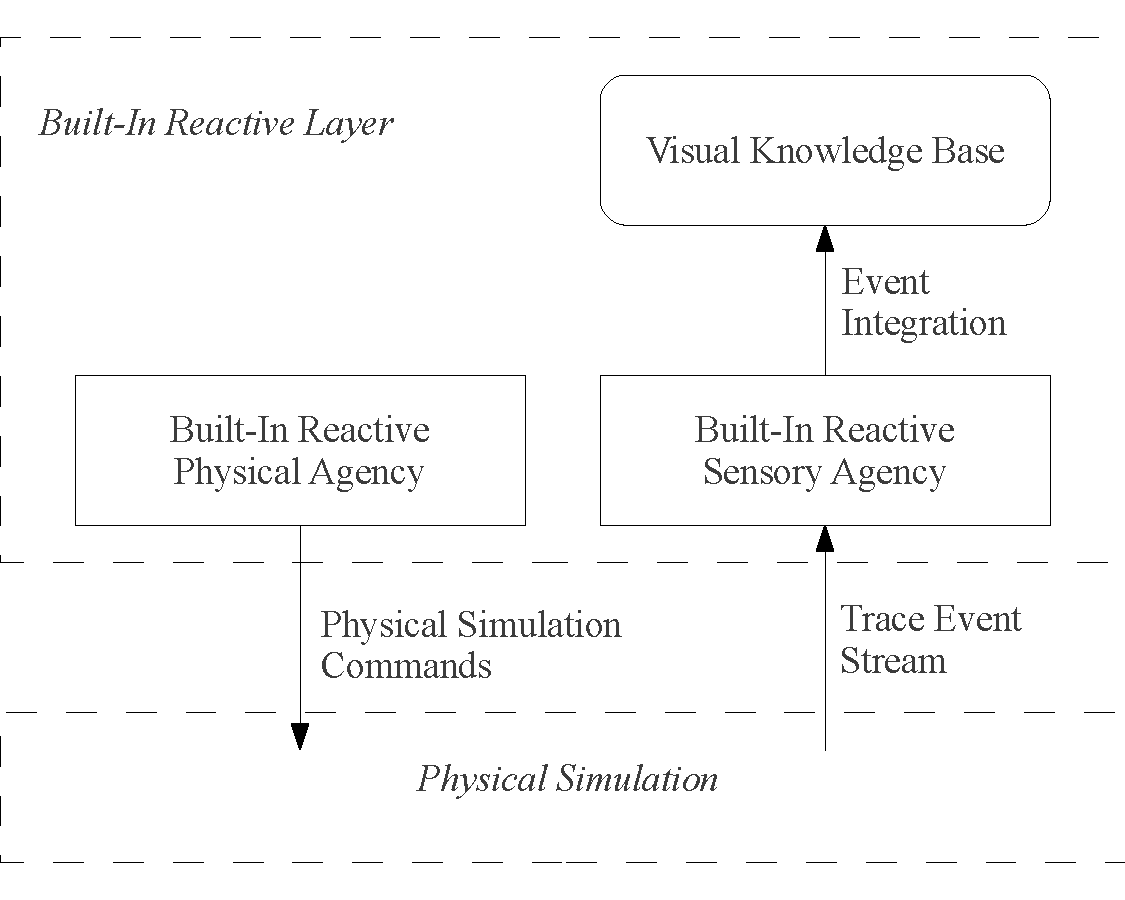
\includegraphics[width=10cm]{gfx/built_in_reactive_and_physical_layers}
\caption{The built-in reactive layer communicates with the physical
  simulation.}
\label{figure:built_in_reactive_and_physical_layers}
\end{figure}
As can be seen in
{\mbox{\autoref{figure:built_in_reactive_and_physical_layers}}}, the
built-in reactive physical and sensory agencies connect the AI to the
physical simulation.  Also shown is the visual knowledge base, the
initial sensory knowledge base in the AI.

\section{The Learned Reactive Layer}

The learned reactive layer in SALS does not have direct access to the
physical simulation.  Instead, the learned reactive layer perceives
the visual knowledge base in the built-in reactive layer and sends
activation or suppression commands to the built-in reactive physical
agency resources.  The learned reactive layer is similar to the
built-in reactive layer because it also contains a {\emph{physical
    agency}}.  However, the learned reactive physical agency contains
resources that execute compiled plans from the deliberative layer
above.  When these resources are activated, they execute plans that
contain sequences of commands that end up either activating or
suppressing built-in reactive resources in the layer below.  Learned
reactive physical resources can fail for a variety of reasons that
will be introduced later when I present the details of plans and the
planning process in
{\mbox{\autoref{chapter:learning_from_being_told}}}.

\subsection{The Physical Knowledge Base}

The learned reactive layer contains an agency called the
{\emph{physical knowledge agency}}.  The physical knowledge agency
contains resources that receive a trace event stream of any changes in
the visual knowledge base.  In partially observable environments, the
physical knowledge base contains a representations of the physical
world that is larger than the current visual knowledge base may
contain as direct sensory knowledge.  The block stacking domain is not
a partially observable environment, so the physical knowledge base in
this case is simply a reconstructed copy of the visual knowledge base.
However, in IsisWorld {\cite[]{smith:2010}}, the partially observable
physical problem domain,
% shown in
%{\mbox{\autoref{figure:isis_world_two_agents_labelled}}},
SALS utilizes the distinction between visual and physical knowledge as
the physical knowledge base is larger than the partial view of
knowledge provided by the visual knowledge base.  In this
dissertation, I will not describe the larger number of different types
of objects with more complex relationships and properties that occur
in the IsisWorld physical simulation.  Because my focus is on learning
to plan and learning to reflectively plan, the visual and physical
details of the IsisWorld simulation would only confuse my point.
%\begin{figure}
%\centering
%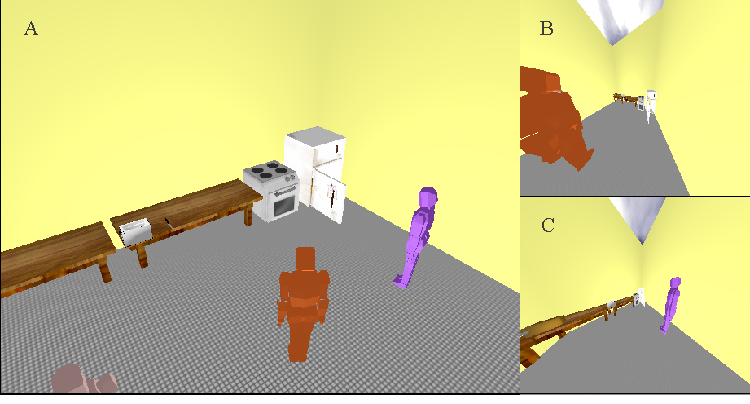
\includegraphics[width=12cm]{gfx/isis_world_two_agents_labelled}
%\caption[IsisWorld physical simulation with two humanoid robots in a
%  partially observable physical problem domain.]{IsisWorld physical
%  simulation with two humanoid robots in a partially observable
%  physical problem domain.  (A) An overview of the entire physical
%  simulation from an omniscient perspective.  (B, C) Each robot only
%  sees a partial perspective of the entire physical domain, depending
%  on each robot's visual perspective.}
%\label{figure:isis_world_two_agents_labelled}
%\end{figure}

\begin{figure}
\centering
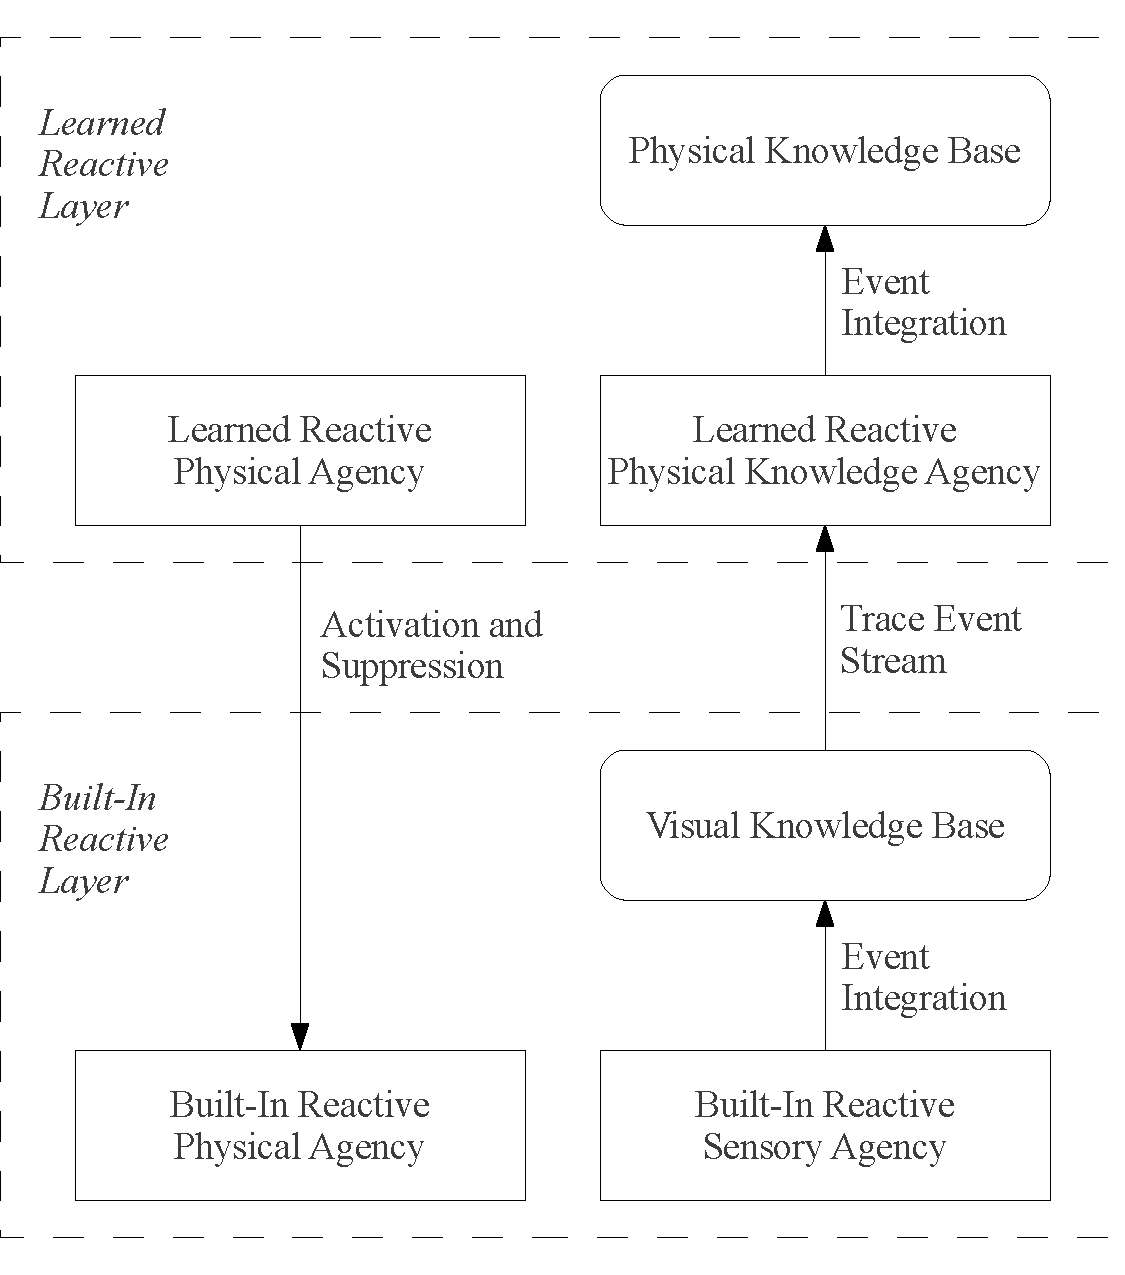
\includegraphics[width=10cm]{gfx/learned_reactive_and_built_in_reactive_layers}
\caption{The learned reactive layer communicates with the built-in
  reactive layer.}
\label{figure:learned_reactive_and_built_in_reactive_layers}
\end{figure}
As can be seen in
{\mbox{\autoref{figure:learned_reactive_and_built_in_reactive_layers}}},
the learned reactive physical and physical knowledge agencies connect
the higher layers of the AI to the built-in reactive layer.  Also
shown is the physical knowledge base, the focus knowledge base that
the deliberative planning layer attempts to accomplish goals within.

The basic mechanism for perceptual abstraction in SALS is based on an
object called a {\emph{partial state}}.  Because all knowledge in SALS
is represented as frames with slots, these knowledge bases can be
simultaneously represented as semantic graphs with objects and their
symbolic properties as nodes of the graph, while slot names are
considered the edges of the graph.
{\mbox{\autoref{figure:physical_knowledge_base_graph}}} shows a graph
representation for the physical knowledge base.  Given this graph
representation of any SALS knowledge base, a partial state of a SALS
knowledge base is any subgraph of one of these knowledge base graphs.
The details of specific partial state object definitions and how the
partial state abstraction process works, while avoiding the complexity
of a general graph matching algorithm are described in
{\mbox{\autoref{chapter:learning_asynchronously_from_experience}}}.
\begin{figure}
\centering
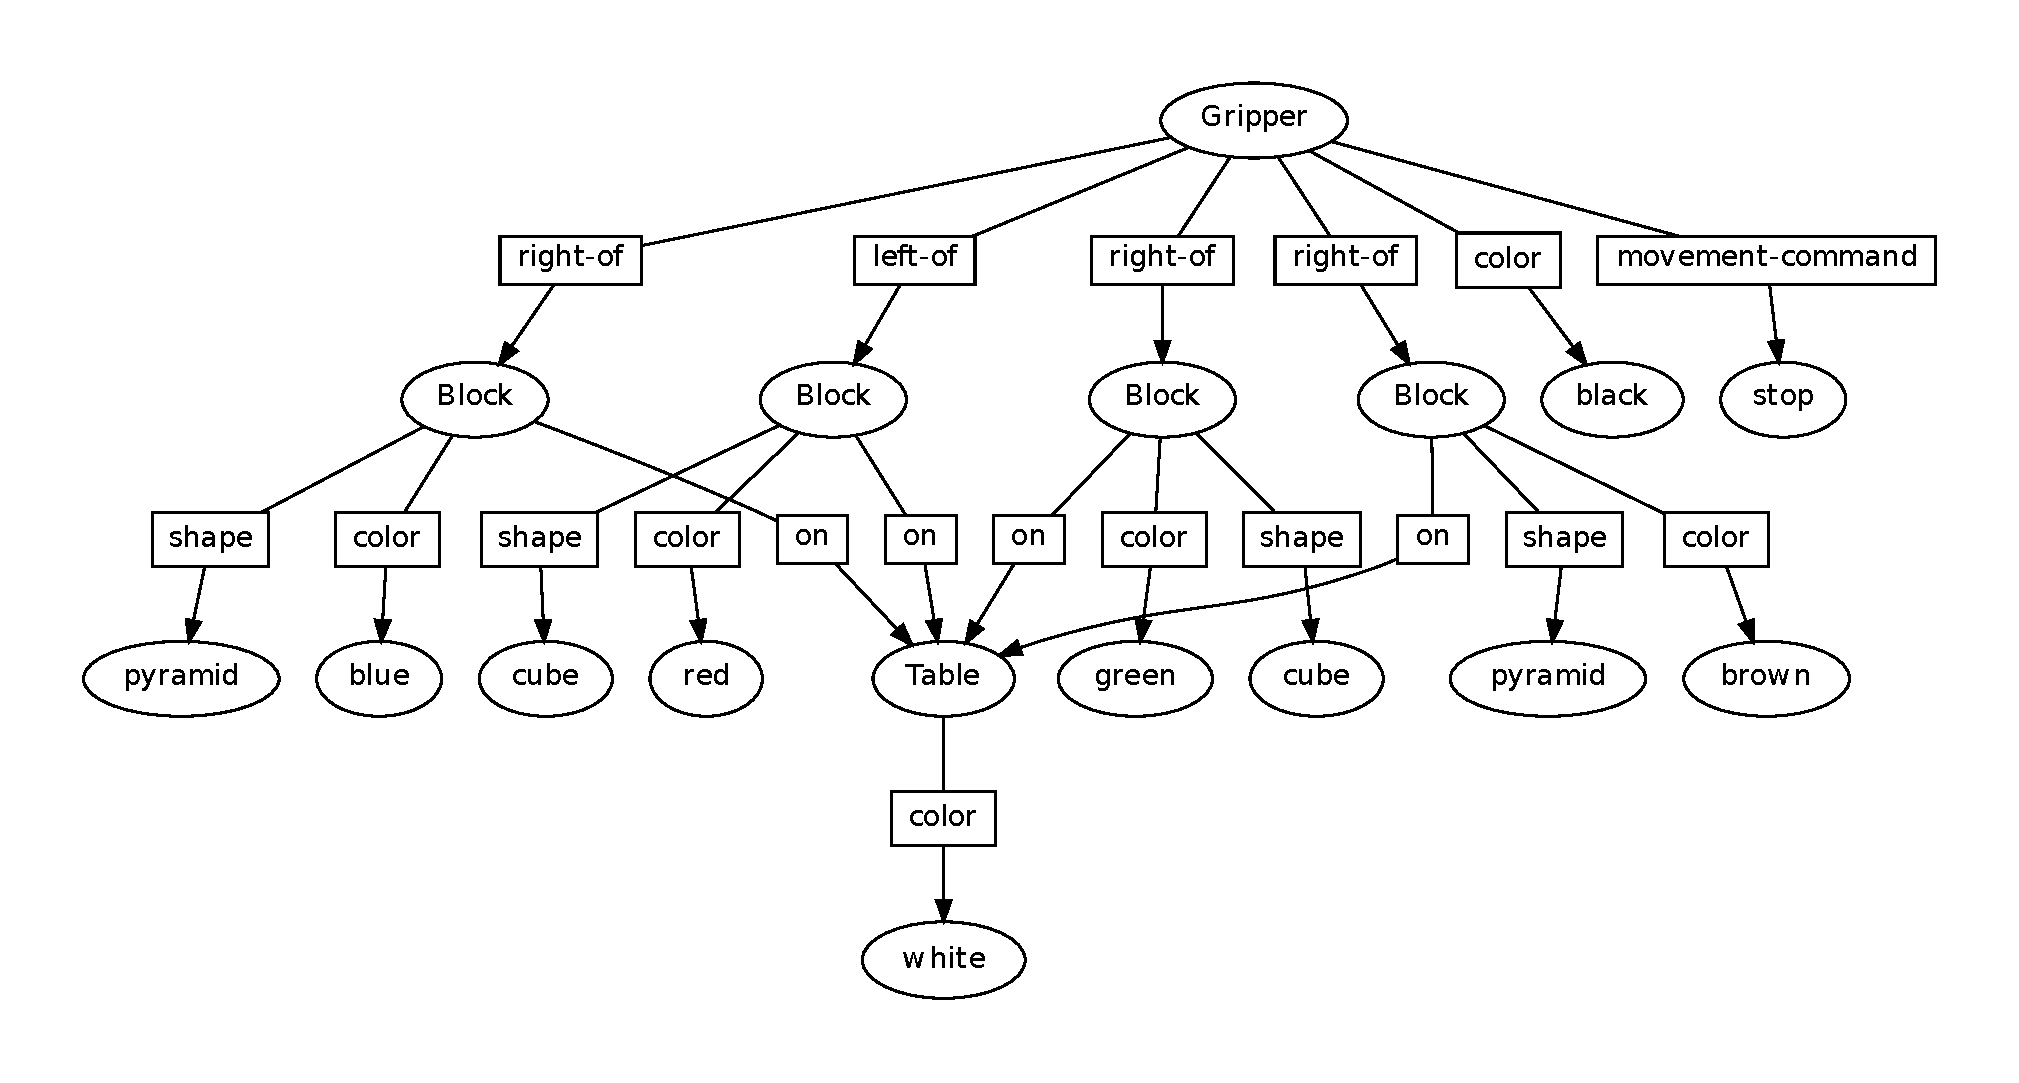
\includegraphics[width=14cm]{gfx/physical_knowledge_base_graph}
\caption[A graph representation of the physical knowledge base.]{A
  graph representation of the physical knowledge base, where
  frame-based objects become interconnected collections of elliptical
  node labels and rectangular edge labels.  This representation is
  consistent with the physical situation shown previously on
  {\mbox{page~\pageref{figure:introduction_example_problem_domain__duplicate_1}}}
  in
  {\mbox{\autoref{figure:introduction_example_problem_domain__duplicate_1}}}.}
\label{figure:physical_knowledge_base_graph}
\end{figure}

\section{The Deliberative Layer}
\label{section:the_deliberative_layer}

The deliberative layer is the first planning layer in the SALS
cognitive architecture.  The deliberative layer tries to accomplish
goals that are partial states of the physical knowledge base in the
learned reactive layer.
{\mbox{\autoref{figure:deliberative_and_learning_reactive_layers}}}
shows an overview of the deliberative layer and its connections to the
learned reactive layer below.  The following are functional
explanations of the labeled parts, A--G, in
{\mbox{\autoref{figure:deliberative_and_learning_reactive_layers}}}:
\begin{figure}
\hspace{-3cm}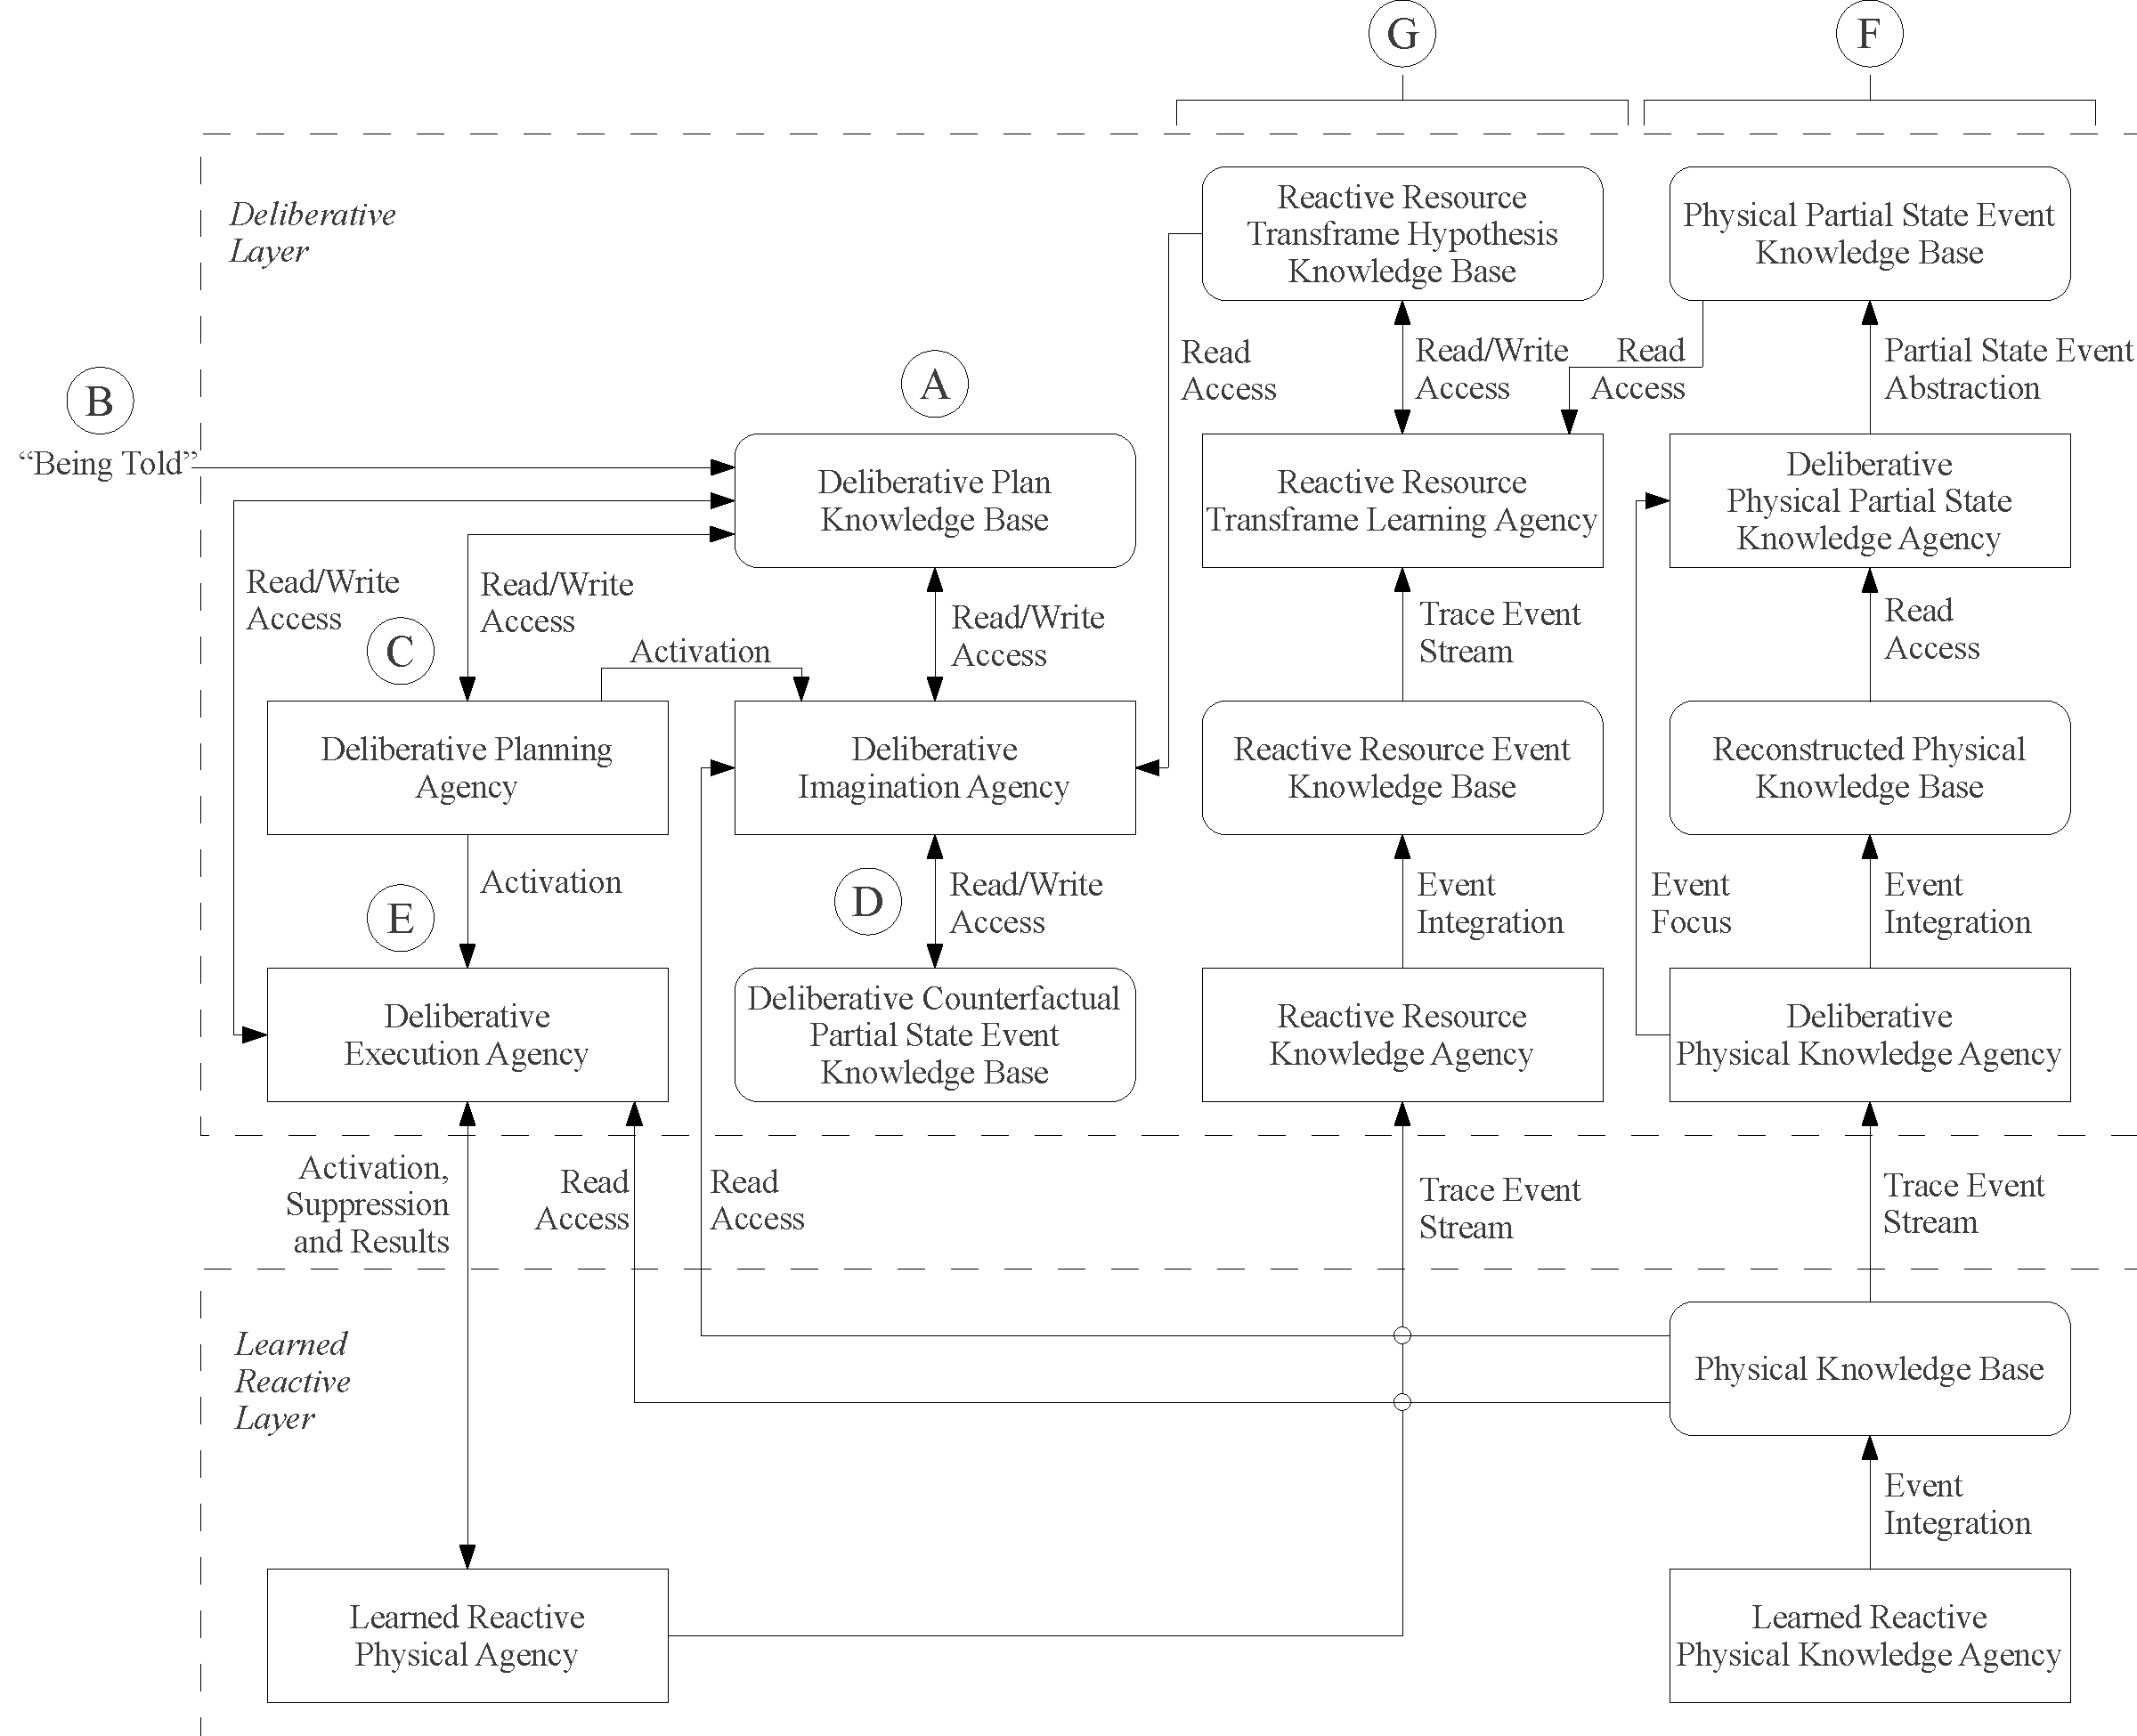
\includegraphics[width=16cm]{gfx/deliberative_and_learned_reactive_layers}
\caption[The deliberative layer and its connections to the learned
  reactive layer.]{The deliberative layer and its connections to the
  learned reactive layer.  See text in
  {\mbox{\autoref{section:the_deliberative_layer}}} for descriptions
  of labeled functional areas, A--G.}
\label{figure:deliberative_and_learning_reactive_layers}
\end{figure}
\begin{enumerate}[~~A.]
\item Natural language plans can enter the {\emph{deliberative plan
    knowledge base}} from outside of the AI by ``being told'' by a
  human user or another AI.  One such natural language plan that has
  been told to the SALS AI is to ``{\tt{stack a cube on a pyramid}}.''
\item The {\emph{deliberative plan knowledge base}} is where all
  deliberative natural language plans for physical action are stored
  along with the state of the deliberative planning machine and plan
  failures.  When natural language plans are told to the deliberative
  layer of the SALS AI, the plan is stored in the deliberative plan
  knowledge base.  When plans are manipulated and new plans are
  created, these new plans are also stored in the deliberative plan
  knowledge base.  In the example story presented in
  {\mbox{\autoref{chapter:introduction}}}, the deliberative planning
  machine focuses on a plan to ``{\tt{stack a cube on pyramid}}.''  At
  this point in the example story, the fact that the deliberative
  planning machine is focused on this plan is also stored as knowledge
  in the deliberative plan knowledge base: ``{\tt{a}}
  {\tt{deliberative}} {\tt{planning}} {\tt{machine}} {\tt{is}}
  {\tt{focused}} {\tt{on}} {\tt{a}} {\tt{plan}} {\tt{to}} {\tt{stack}}
  {\tt{a}} {\tt{cube}} {\tt{on}} {\tt{a}} {\tt{pyramid}}.''  Details
  of the internal representation of the deliberative plan knowledge
  base will be described in
  {\mbox{\autoref{section:the_deliberative_plan_knowledge_base}}}.
  The state of the deliberative plan knowledge base is reflected upon
  by the reflective layer, which will be described in
  {\mbox{\autoref{section:the_reflective_layer}}}.
\item The {\emph{deliberative planning agency}} contains the resources
  for planning activities that manipulate plans in the deliberative
  plan knowledge base as well as resources that in turn activate the
  resources in the neighboring deliberative imagination and execution
  agencies.  The deliberative planning agency includes resources that
  cause the imagination of the effects of a plan in focus, change the
  planning focus, manipulate plans currently in focus, as well as
  cause the execution of plans currently in focus.  The reflective
  layer, described in {\mbox{\autoref{section:the_reflective_layer}}},
  activates the resources in the deliberative planning agency to
  control the deliberative planning machine.
\item The {\emph{deliberative imagination agency}} imagines the
  hypothetical future effects of executing deliberative plans for
  physical action.  The {\emph{deliberative counterfactual partial
      state event knowledge base}} is used as a scratchpad for storing
  these hypothetical future physical states.  The current state of the
  physical knowledge base in the layer below is used as a starting
  point for the counterfactual knowledge created by the deliberative
  imagination agency.  For example, when the deliberative planning
  agency focuses the planning machine on the plan to ``{\tt{stack a
      cube on a pyramid}}'' and subsequently activates the
  deliberative imagination agency, the effects of the plan are
  imagined and the deliberative counterfactual partial state event
  knowledge base subsequently contains the physical partial state for
  ``{\tt{a cube to be on a pyramid}}.''
\item The {\emph{deliberative execution agency}} executes plans by
  activating and suppressing resources in the learned reactive
  physical agency in the layer below.  For example, when the
  deliberative planning agency focuses the planning machine on the
  plan to ``{\tt{stack a cube on a pyramid}}'' and subsequently
  activates the deliberative execution agency, the body of the plan is
  executed, including activating resources in the physical agency to
  ``{\tt{move right}},'' ``{\tt{grab}},'' ``{\tt{move left}},'' and
  ``{\tt{drop}}.''
\item A column of agencies and knowledge bases abstract partial states
  from the physical knowledge base in the learned reactive layer
  below.  Because partial state abstraction can be a slow process,
  this process is performed asynchronously based on a stream of change
  events.  A detailed description of partial states and their
  asynchronous abstraction will be given in
  {\mbox{\autoref{chapter:learning_asynchronously_from_experience}}},
  {\mbox{\autoref{section:partial_state_event_abstraction}}}.
  Abstracted partial state event knowledge is stored in the
  {\emph{physical partial state event knowledge base}}.  The
  abstraction of partial states is one of two types of asynchronous
  processing streams that constitute the SALS AI's ability to learn
  from the experience of executing plans.
\item A column of agencies and knowledge bases perform asynchronous
  learning of abstract causal rule hypotheses from physical agency
  resource execution preconditions.  The advantage of an asynchronous
  learning algorithm is that it does not slow down the execution of
  plans in the deliberative layer.  Historical versions of knowledge
  bases are reconstructed so that the slower learning algorithms can
  discover relevant patterns in this data for predicting the effects
  of actions.  For example, when the deliberative execution agency
  executes the plan ``{\tt{stack a cube on a pyramid}},'' the SALS AI
  learns that when ``{\tt{a gripper is holding a cube}}'' and ``{\tt{a
      pyramid is below a gripper}},'' the resulting state will
  {\emph{not}} be ``{\tt{a cube is on a pyramid}}.''  The details of
  the asynchronous learning of abstract causal rules from the
  experience of executing plans will be described in
  {\mbox{\autoref{chapter:learning_asynchronously_from_experience}}},
  {\mbox{\autoref{section:resource_execution_event_causal_rule_learning}}}.
\end{enumerate}

\subsection{The Deliberative Plan Knowledge Base}
\label{section:the_deliberative_plan_knowledge_base}

The {\emph{deliberative plan knowledge base}} is the heart of the
deliberative layer, where all deliberative natural language plans for
physical action are stored along with the deliberative planning
machine and deliberative plan failures.  Natural language plans can
enter the deliberative plan knowledge base from outside of the AI by
``being told,'' which is a form of natural language programming,
possibly in the form of an natural language expression from the user.
The {\emph{deliberative planning agency}} is the center of executive
control in the deliberative layer.  The deliberative planning agency
manipulates plans and also activates the {\emph{deliberative
    imagination agency}} and the {\emph{deliberative execution
    agency}} when these plans should be imagined or executed.  The
deliberative imagination agency uses learned rules that map
preconditions of learned reactive physical agency resource activations
to changes that these resources cause to occur in the learned reactive
physical knowledge base.  The deliberative imagination agency uses the
{\emph{deliberative counterfactual partial state event knowledge
    base}} as a scratchpad that can store hypothetical future states
of the learned reactive physical knowledge base if the appropriate
learned reactive physical agency resources are activated.  Once the
deliberative planning agency has decided to execute a given plan, the
deliberative execution agency is activated, which executes plans by
activating and suppressing resources in the learned reactive physical
agency in the layer below.

Similar to the visual and physical knowledge bases, the deliberative
plan knowledge base also consists of collections of interconnected
frame-based objects.  The following are different possible property
slots and symbolic values for the deliberative objects in the
deliberative plan knowledge base:
\begin{samepage}
  \begin{packed_itemize}
  \item{{\emph{type}}: $\{$``{\tt{plan}}'', ``{\tt{planner}}'', ``{\tt{execution-node}}'', ``{\tt{failure}}''$\}$}
  \item{{\emph{has-been-imagined}}: $\{$``{\tt{true}}'', ``{\tt{false}}''$\}$}
  \item{{\emph{default-slot-value}}: $\{$all natural language strings$\}$}
  \item{{\emph{hypothesized-to-cause}}: $\{$all physical partial states$\}$}
  \item{{\emph{positive-goal}}: $\{$all physical partial states$\}$}
  \item{{\emph{negative-goal}}: $\{$all physical partial states$\}$}
  \end{packed_itemize}
\end{samepage}
These properties are examples of those aspects of the deliberative
thinking layer that the AI can reflectively see about a single
deliberative object, including the type, the default slot values of a
natural language plan, and the goals of a planner.  In addition to
each deliberative object having properties, each deliberative object
may have different types of relations to other deliberative objects
that the AI can reflectively perceive.  Some are these relations are
as follows:
\begin{samepage}
  \begin{packed_itemize}
  \item{\emph{focus-plan}}
  \item{\emph{execution-plan}}
  \item{\emph{imagination-failure}}
  \item{\emph{execution-failure}}
  \item{\emph{start-execution-node}}
  \item{\emph{previous}}
  \item{\emph{next}}
  \item{\emph{subnode}}
  \item{\emph{supernode}}
  \end{packed_itemize}
\end{samepage}
I will describe the details of the objects in the deliberative plan
knowledge base in {\mbox{\autoref{chapter:learning_from_being_told}}},
where I will describe learning from being told and the natural
language planning process.  A simplified graph representation of the
deliberative plan knowledge base is shown in
{\mbox{\autoref{figure:deliberative_plan_knowledge_base_graph}}}.
\label{page:deliberative_plan_knowledge_base_graph-label_descriptions}
\begin{figure}
\hspace{0cm}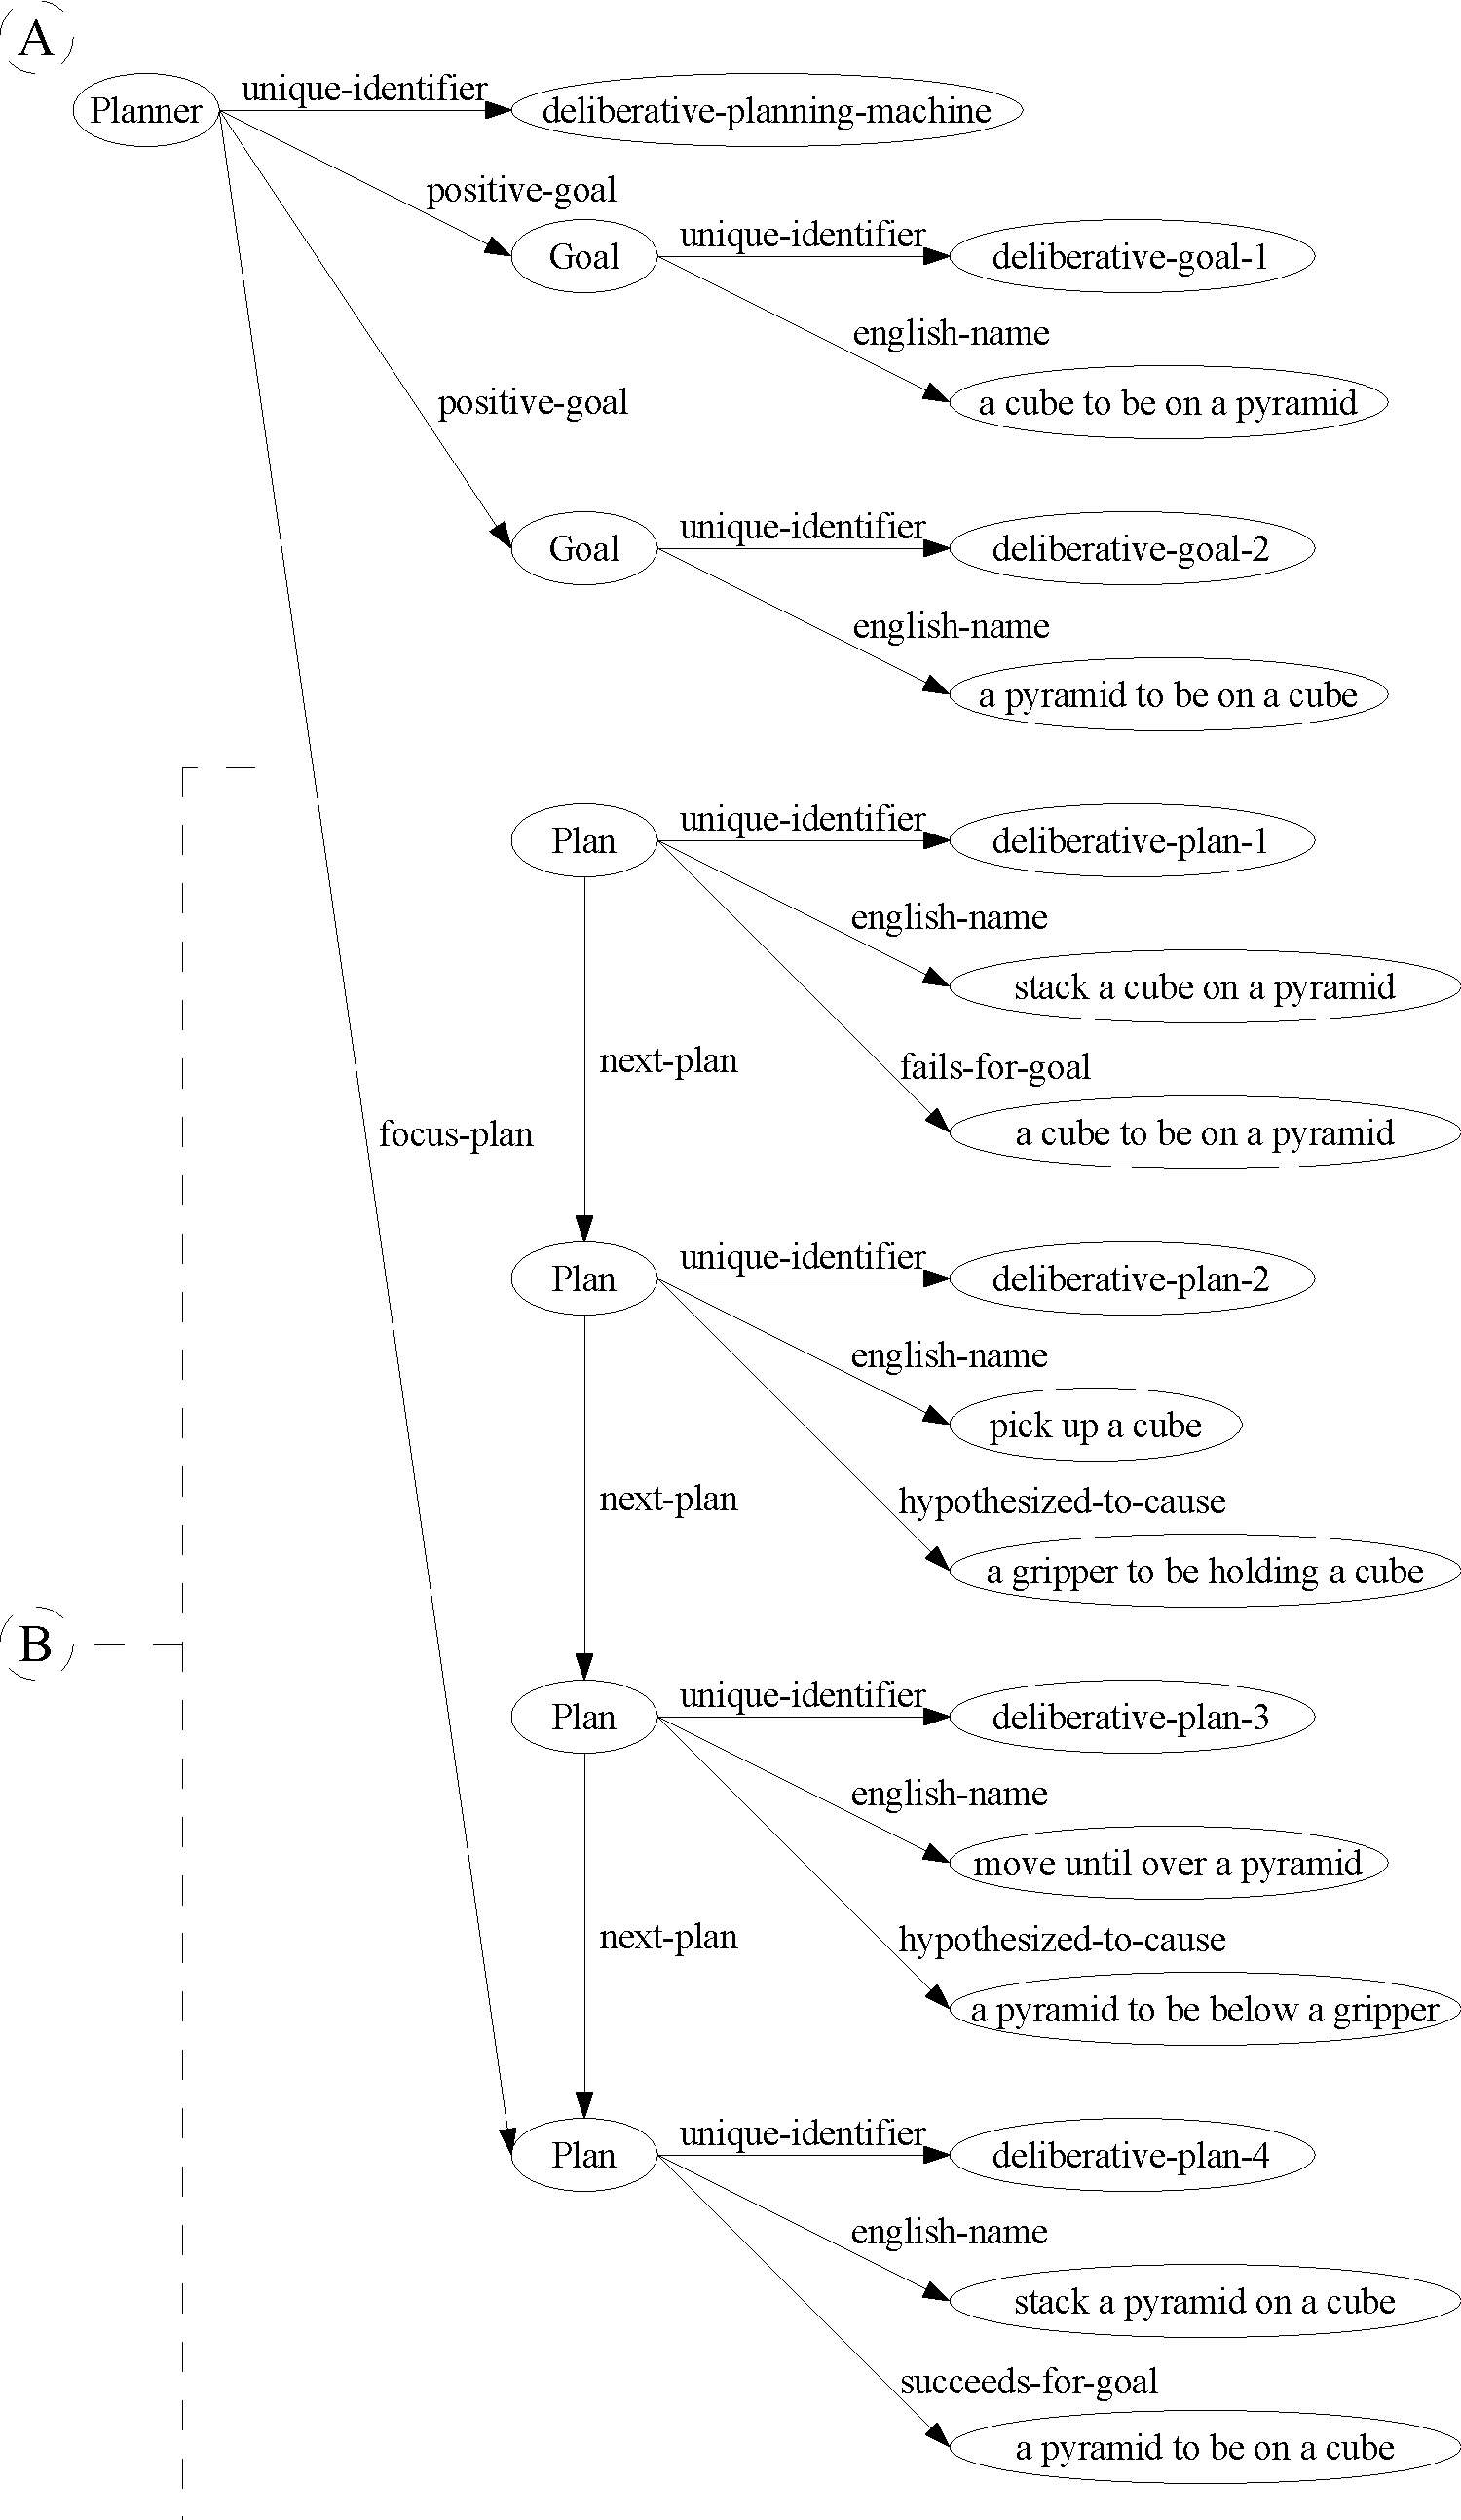
\includegraphics[height=20cm]{gfx/deliberative_plan_knowledge_base_graph-handdrawn}
\caption[Part of the deliberative plan knowledge base represented as a
  graph.]{Part of the deliberative plan knowledge base represented as
  a graph.  See text in
  {\mbox{\autoref{section:the_deliberative_plan_knowledge_base}}} on
  {\mbox{page~\pageref{page:deliberative_plan_knowledge_base_graph-label_descriptions}}}
  for descriptions of knowledge labels, {\mbox{A~and~B}}.}
\label{figure:deliberative_plan_knowledge_base_graph}
\end{figure}
In this figure, knowledge labels {\mbox{A~and~B}} refer to the
following different types of deliberative knowledge:
\begin{enumerate}[~~A.]
\item The state of the {\emph{deliberative planning machine}} includes
  positive and negative physical goals as well as references to plans
  for physical action that the planning machine is currently focusing
  on or executing.  For example, in the story presented in
  {\mbox{\autoref{chapter:introduction}}}, the plan to ``{\tt{want a
      block to be on a block}}'' is a reflective plan that has
  previously been told to the reflective layer of the SALS AI.  The
  execution of this reflective plan causes the deliberative planning
  machine to be given two specific positive goals for either ``{\tt{a
      cube to be on a pyramid}}'' or ``{\tt{a pyramid to be on a
      cube}}.''  At the end of the story, the reflective SALS AI
  successfully accomplishes its goal for ``{\tt{a pyramid to be on a
      cube}}'' by first focusing on the last plan that it has been
  told and then executing this plan.
\item Representations of deliberative plans are organized into a
  linked-list structure that goes forward and backward in time.  Plans
  that have been told to the SALS AI furthest in the past are at the
  beginning of the list.  In the example story, the SALS AI uses this
  linked-list structure to organize its search through deliberative
  plans for physical action.  Initially, the SALS AI considers plans
  from newest to oldest, which results in finding the plan,
  ``{\tt{stack a cube on a pyramid}},'' which fails to accomplish its
  goal for ``{\tt{a cube to be on a pyramid}}.''  Finally, the SALS AI
  searches through deliberative plans from oldest to newest and this
  results in finding the plan, ``{\tt{stack a pyramid on a cube}},''
  which succeeds in accomplishing its goal for ``{\tt{a pyramid to be
      on a cube}}.''  At this point in the example, the SALS AI
  reflectively learns to apply a different planning method for the
  current goals of the deliberative planning machine.
\end{enumerate}
%% \begin{sidewaysfigure}
%% \begin{center}
%% \includegraphics[width=8.5in]{gfx/deliberative_plan_knowledge_base_graph}
%% \end{center}
%% \hspace{4cm}\parbox{15cm}{\caption[A simplified graph representation
%%     of the deliberative plan knowledge base.]{A simplified graph
%%     representation of the deliberative plan knowledge base, where
%%     frame-based objects become interconnected collections of
%%     elliptical node labels and rectangular edge labels.  The
%%     deliberative planner node is at the top of the graph.  This
%%     planner is ``focused'' on a linked list of deliberative plan
%%     objects.  The planner has two goals: (1) ``{\tt{a pyramid to be on
%%         a cube}},'' and (2) ``{\tt{a cube to be on a pyramid}}.''  The
%%     causal effects of the first plan have been imagined and are listed
%%     as properties of the plan object.  The execution node structure of
%%     the deliberative imagination process are not shown for visual
%%     simplicity.}\label{figure:deliberative_plan_knowledge_base_graph}}
%% \end{sidewaysfigure}

\subsection{Asynchronous Learning}

To imagine the effects of executing plans, the deliberative layer
learns abstract hypothetical models of the effects of learned reactive
physical agency resource activations.  These learned models are
generated by a rule learning algorithm that predicts a hypothetical
{\emph{transframe}} \cite[]{minsky:1975} given the preconditions for
an action.  Transframes represent changes between one collection of
frames and another collection of frames.  The details of transframes
in the SALS AI will be discussed in
{\mbox{\autoref{chapter:learning_asynchronously_from_experience}}},
{\mbox{\autoref{section:resource_execution_event_causal_rule_learning}}}.
Asynchronous learning is implemented as two stages of stream
processing.  The first stage abstracts partial state events from a
trace event stream composed of any change events that occur in the
learned reactive physical knowledge base.  The second stage receives a
stream of activation and completion events from the learned reactive
physical agency resources.  Because both of these asynchronous stages
process different types of event streams at different rates, the
resulting knowledge bases are accurate for different points of time in
the past.  Although the timing of the two-staged asynchronous learning
in SALS complicates the implementation, the advantage is simple: the
execution of learned reactive physical agency resources and the
manipulation of the learned reactive physical knowledge base can both
operate at full speed, while the slower learning algorithm can operate
at its own pace.  In practice, resource activations and knowledge
changes occur in high-speed bursts, followed by periods of
deliberation, which generally gives the slower learning algorithms
time to catch up.  The details of the SALS asynchronous learning
algorithm will be discussed in
{\mbox{\autoref{chapter:learning_asynchronously_from_experience}}}.

\section{The Reflective Layer}
\label{section:the_reflective_layer}

While the deliberative layer focuses on learning the effects of
physical actions to make plans to control the physical knowledge base,
the reflective layer focuses on learning the effects of deliberative
planning actions to make plans to control the deliberative plan
knowledge base.  This similarity is abstracted in SALS and is called a
{\emph{planning layer}}.  The deliberative, reflective, and
super-reflective layers are all instantiations of these planning layer
cognitive architectural objects.  A planning layer is an extension
that can be added to any paired combination of a knowledge base and an
agency of resources to learn how to use to control the partial states
within the knowledge base.
{\mbox{\autoref{figure:reflective_and_deliberative_layers}}} shows the
reflective layer and its connection to the deliberative layer.  While
the deliberative layer focuses on learning about making plans to
control the physical knowledge base, the reflective layer focuses on
learning about making plans to control the deliberative plan knowledge
base.  This similarity is abstracted in SALS and is called a
{\emph{planning layer}}.  The deliberative, reflective, and
super-reflective layers are all instantiations of these planning layer
cognitive architectural objects.
\begin{figure}
\hspace{-3cm}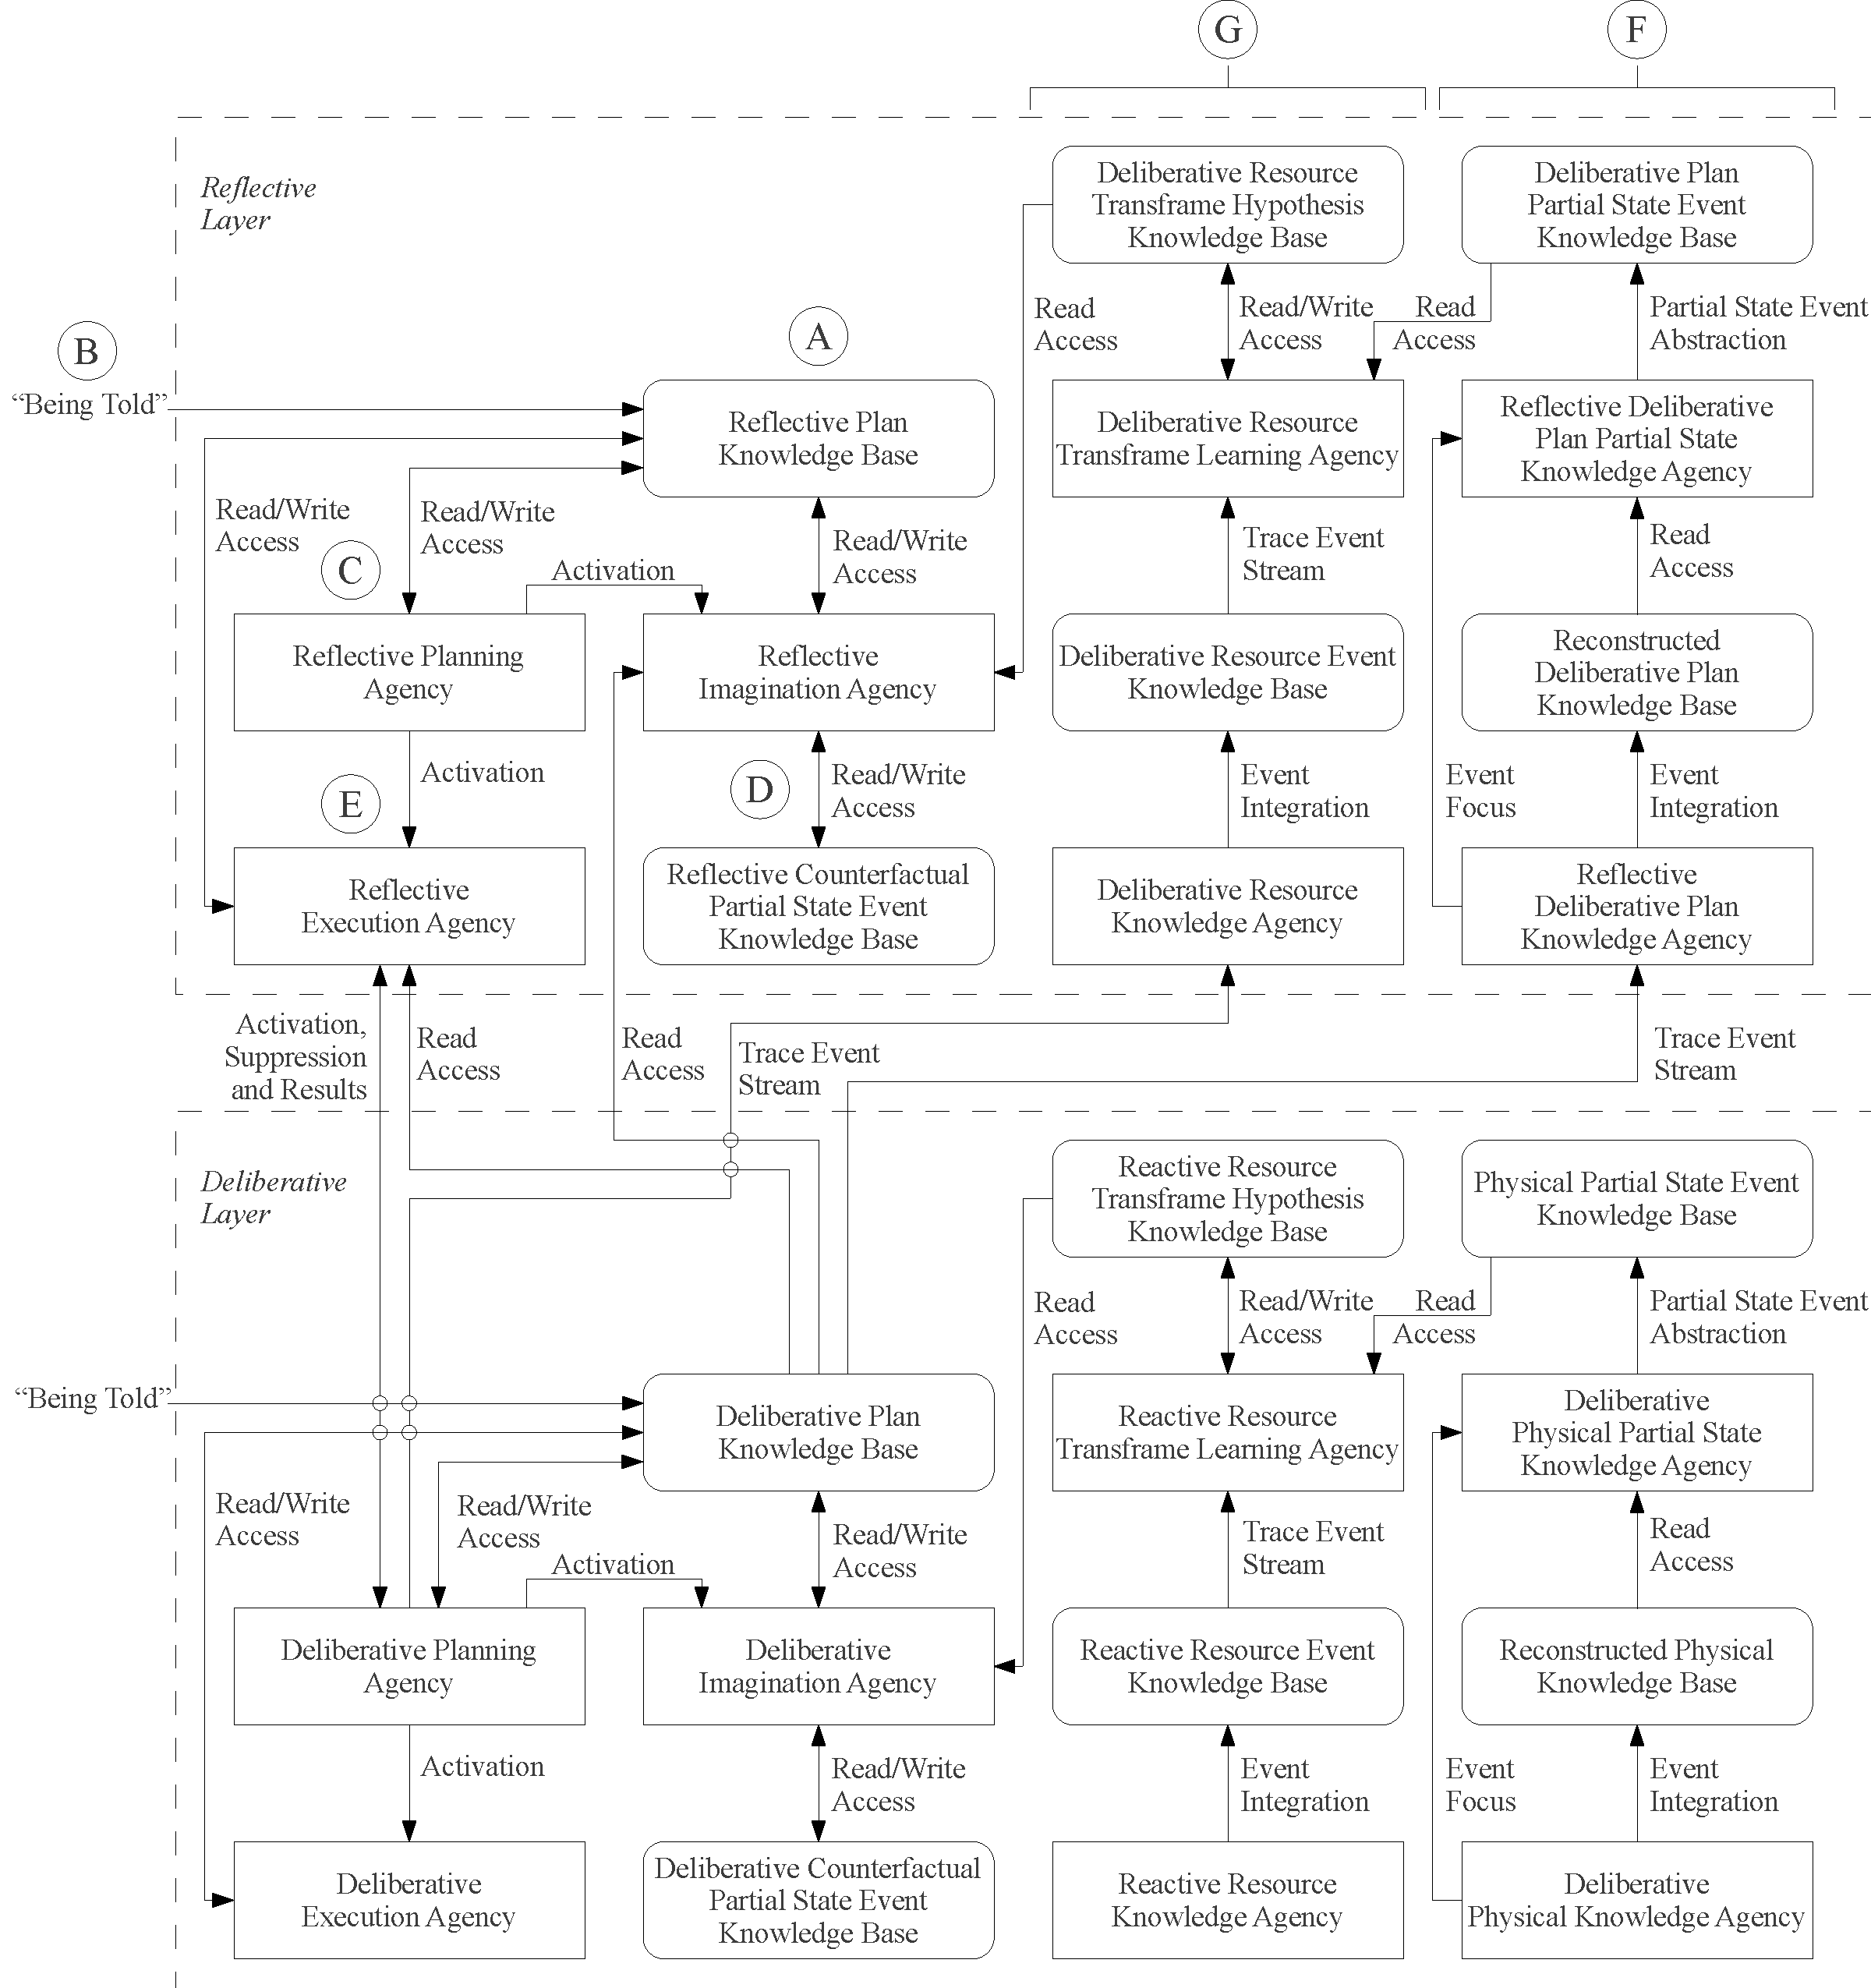
\includegraphics[width=16cm]{gfx/reflective_and_deliberative_layers}
\caption[The reflective layer and its connection to the deliberative
  layer.]{The reflective layer and its connection to the deliberative
  layer is analogous to the deliberative layer and its connection to
  the learned reactive layer, shown in
  {\mbox{\autoref{figure:physical_knowledge_base_graph}}} on
  {\mbox{page~\pageref{figure:physical_knowledge_base_graph}}}.  See
  text in {\mbox{\autoref{section:the_reflective_layer}}} for
  descriptions of labeled functional areas, A--G.}
\label{figure:reflective_and_deliberative_layers}
\end{figure}
\begin{enumerate}[~~A.]
\item Natural language plans can enter the {\emph{reflective plan
    knowledge base}} from outside of the AI by ``being told'' by a
  human user or another AI.  One such reflective natural language plan
  that has been told to the SALS AI in the example presented in
  {\mbox{\autoref{chapter:introduction}}} is to ``{\tt{find an old
      plan to accomplish a goal}}.''  Plans in the reflective plan
  knowledge base include different methods for how to find or create
  plans to accomplish different types of physical partial states, or
  deliberative goals.
\item The {\emph{reflective plan knowledge base}} is where all
  reflective natural language plans for deliberative action are stored
  along with the state of the reflective planning machine and
  reflective plan failures.  When natural language plans are told to
  the reflective layer of the SALS AI, the plan is stored in the
  reflective plan knowledge base.  In the example story presented in
  {\mbox{\autoref{chapter:introduction}}}, the reflective planning
  machine focuses on a plan to ``{\tt{find a recent plan to accomplish
      a goal}}.''  At this point in the example story, the fact that
  the reflective planning machine is focused on this plan is also
  stored as knowledge in the reflective plan knowledge base:
  ``{\tt{a}} {\tt{reflective}} {\tt{planning}} {\tt{machine}}
  {\tt{is}} {\tt{focused}} {\tt{on}} {\tt{a}} {\tt{plan}} {\tt{to}}
  {\tt{find}} {\tt{a}} {\tt{recent}} {\tt{plan}} {\tt{to}}
  {\tt{accomplish}} {\tt{a}} {\tt{goal}}.''  Details of the internal
  representation of the reflective plan knowledge base will be
  described in
  {\mbox{\autoref{section:the_reflective_plan_knowledge_base}}}.  The
  state of the reflective plan knowledge base is further reflected
  upon by the super-reflective layer, which will be described in
  {\mbox{\autoref{section:the_super_reflective_layer}}}.
\item The {\emph{reflective planning agency}} contains the resources
  for reflective planning activities that manipulate plans in the
  reflective plan knowledge base as well as resources that in turn
  activate the resources in the neighboring reflective imagination and
  execution agencies.  The reflective planning agency includes
  resources that cause the imagination of the effects of a reflective
  plan in focus, change the reflective planning focus, manipulate
  reflective plans currently in focus, as well as cause the execution
  of reflective plans currently in focus.  The super-reflective layer,
  described in {\mbox{\autoref{section:the_super_reflective_layer}}},
  activates the resources in the reflective planning agency to control
  the reflective planning machine.
\item The {\emph{reflective imagination agency}} imagines the
  hypothetical future effects of executing reflective plans for
  deliberative action.  The {\emph{reflective counterfactual partial
      state event knowledge base}} is used as a scratchpad for storing
  these hypothetical future deliberative states.  The current state of
  the deliberative plan knowledge base in the layer below is used as a
  starting point for the counterfactual knowledge created by the
  reflective imagination agency.  For example, when the reflective
  planning agency focuses the reflective planning machine on the plan
  to ``{\tt{find a recent deliberative plan to accomplish a goal}}''
  and subsequently activates the reflective imagination agency, the
  effects of the plan are imagined and the reflective counterfactual
  partial state event knowledge base subsequently contains the
  deliberative partial state for ``{\tt{a plan has an expectation
      failure}}.''  This prediction of plan failure does not require
  the deliberative layer to imagine the physical effects of executing
  physical actions; instead, plan failure is predicted reflectively
  from the structure of the deliberative plan and its relationship to
  the deliberative planning machine, including the current
  deliberative goals.
\item The {\emph{reflective execution agency}} executes reflective
  plans by activating and suppressing resources in the deliberative
  plan agency in the layer below.  For example, when the reflective
  planning agency focuses the reflective planning machine on the plan
  to ``{\tt{find a recent deliberative plan to accomplish a goal}}''
  and subsequently activates the reflective execution agency, the body
  of the plan is executed, including activating resources in the
  deliberative plan agency to ``{\tt{focus}} {\tt{on}} {\tt{most}}
  {\tt{recent}} {\tt{plan}},'' ``{\tt{focus}} {\tt{on}}
  {\tt{previous}} {\tt{plan}},'' ``{\tt{imagine}} {\tt{effects}}
  {\tt{of}} {\tt{plan}} {\tt{in}} {\tt{focus}},'' and ``{\tt{execute}}
  {\tt{plan}} {\tt{in}} {\tt{focus}}.''
\item A column of agencies and knowledge bases abstract partial states
  from the deliberative plan knowledge base in the deliberative layer
  below.  Because partial state abstraction can be a slow process,
  this process is performed asynchronously based on a stream of change
  events.  A detailed description of partial states and their
  asynchronous abstraction will be given in
  {\mbox{\autoref{chapter:learning_asynchronously_from_experience}}},
  {\mbox{\autoref{section:partial_state_event_abstraction}}}.
  Abstracted partial state event knowledge is stored in the
  {\emph{deliberative plan partial state event knowledge base}}.  The
  abstraction of partial states is one of two types of asynchronous
  processing streams that constitute the SALS AI's ability to learn
  from the experience of executing plans.
\item A column of agencies and knowledge bases perform asynchronous
  learning of abstract causal rule hypotheses from deliberative plan
  agency resource execution preconditions.  The advantage of an
  asynchronous learning algorithm is that it does not slow down the
  execution of plans in the reflective layer.  Historical versions of
  the deliberative plan knowledge base are reconstructed so that the
  slower learning algorithms in the reflective layer can discover
  relevant patterns in this data for predicting the effects of
  deliberative actions.  For example, when the reflective execution
  agency executes the plan to ``{\tt{find a recent deliberative plan
      to accomplish a goal}},'' the SALS AI learns that when ``{\tt{a
      planner has the goal for a cube to be on a pyramid}}'' and
  ``{\tt{a planner has the goal for a pyramid to be on a cube}},'' the
  resulting state will be ``{\tt{a plan has an expectation
      failure}}.''  The details of the asynchronous learning of
  abstract causal rules from the experience of executing plans will be
  described in
  {\mbox{\autoref{chapter:learning_asynchronously_from_experience}}},
  {\mbox{\autoref{section:resource_execution_event_causal_rule_learning}}}.
\end{enumerate}

\subsection{The Reflective Plan Knowledge Base}
\label{section:the_reflective_plan_knowledge_base}

A simplified graph representation of the reflective plan knowledge
base is shown in
{\mbox{\autoref{figure:reflective_plan_knowledge_base_graph}}}.
\label{page:reflective_plan_knowledge_base_graph-label_descriptions}
\begin{figure}
\hspace*{-2cm}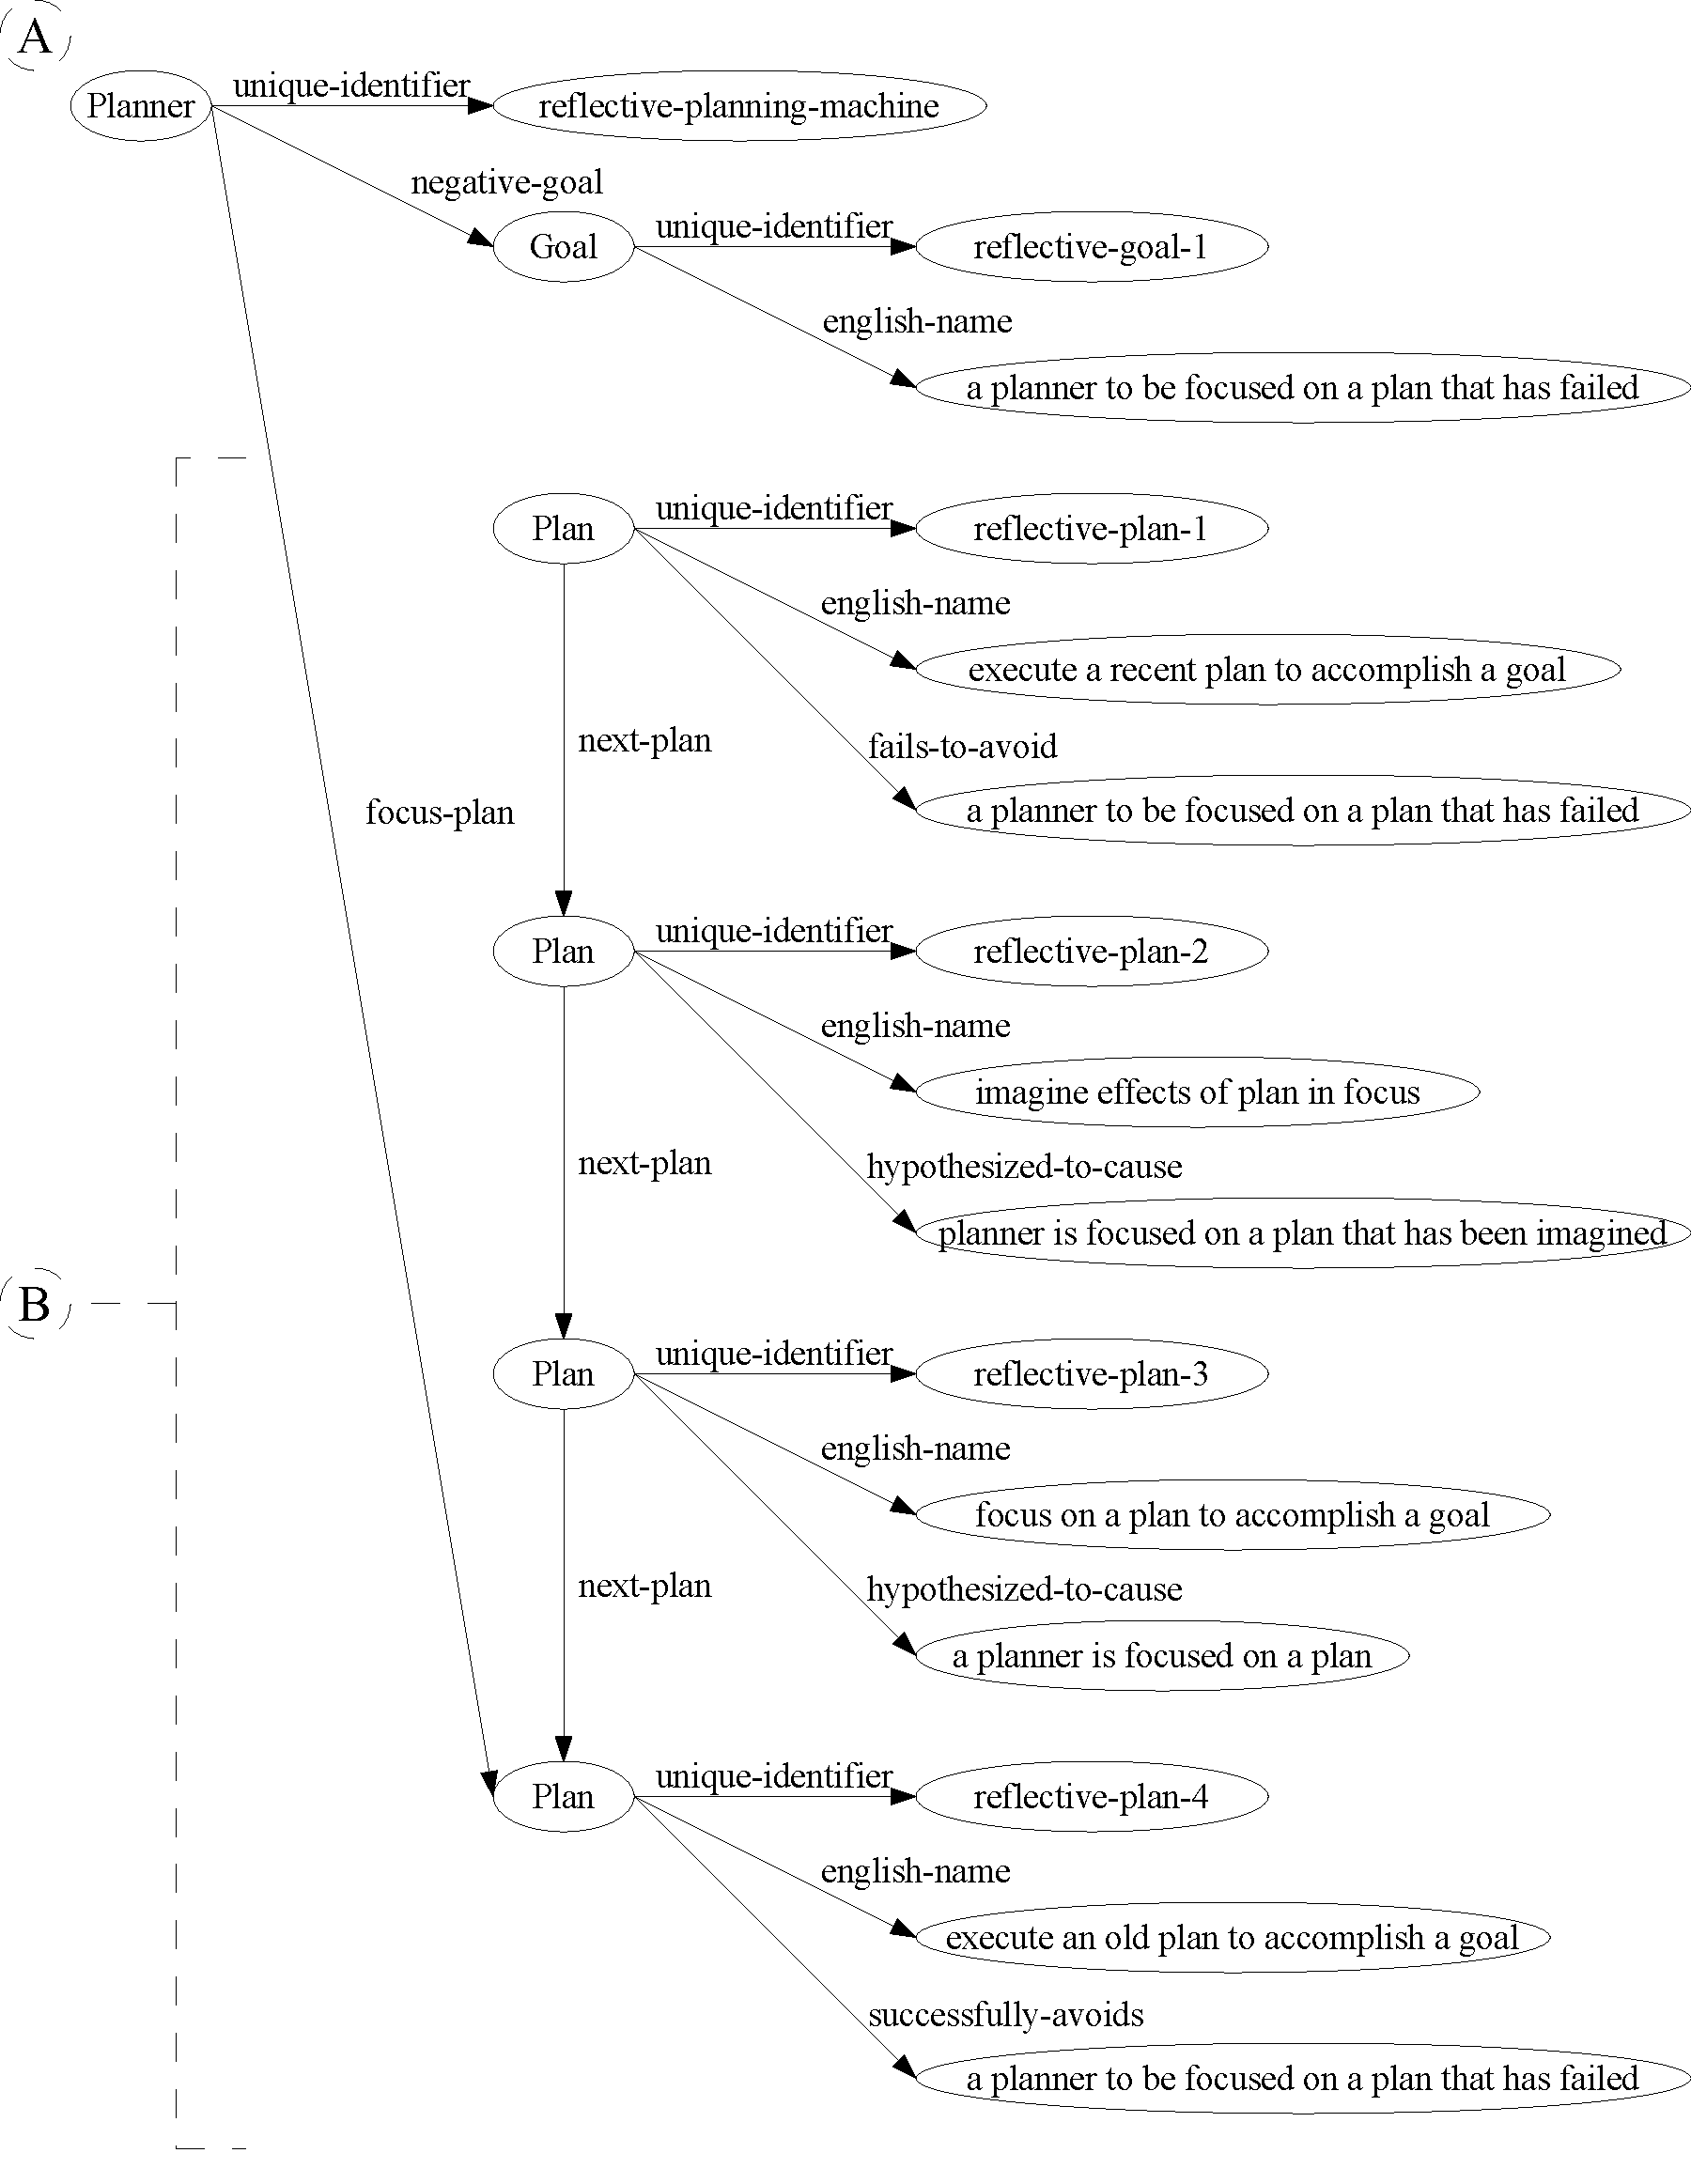
\includegraphics[height=20cm]{gfx/reflective_plan_knowledge_base_graph-handdrawn}
\caption[Part of the reflective plan knowledge base represented as a
  graph.]{Part of the reflective plan knowledge base represented as a
  graph.  See text in
  {\mbox{\autoref{section:the_reflective_plan_knowledge_base}}} on
  {\mbox{page~\pageref{page:reflective_plan_knowledge_base_graph-label_descriptions}}}
  for descriptions of knowledge labels, {\mbox{A~and~B}}.}
\label{figure:reflective_plan_knowledge_base_graph}
\end{figure}
In this figure, knowledge labels {\mbox{A~and~B}} refer to the
following different types of reflective knowledge:
\begin{enumerate}[~~A.]
\item The state of the {\emph{reflective planning machine}} includes
  positive and negative reflective goals as well as references to
  reflective plans for deliberative action.  For example, in the story
  presented in {\mbox{\autoref{chapter:introduction}}}, the reflective
  planning machine has the negative goal for avoiding ``{\tt{a}}
  {\tt{planner}} {\tt{to}} {\tt{be}} {\tt{focused}} {\tt{on}} {\tt{a}}
  {\tt{plan}} {\tt{that}} {\tt{has}} {\tt{failed}}.''  The reflective
  planning machine fails to avoid this deliberative partial state when
  it executes a plan to ``{\tt{execute}} {\tt{a}} {\tt{recent}}
  {\tt{plan}} {\tt{to}} {\tt{accomplish}} {\tt{a}} {\tt{goal}},''
  which leads to a failure while executing the deliberative plan to
  ``{\tt{stack}} {\tt{a}} {\tt{cube}} {\tt{on}} {\tt{a}}
  {\tt{pyramid}}.''
\item Representations of reflective plans are organized into a
  linked-list structure that goes forward and backward in time.  Plans
  that have been told to the SALS AI furthest in the past are at the
  beginning of the list.  In the example story, the SALS AI uses this
  linked-list structure to organize its search through reflective
  plans for deliberative action.  Initially, the SALS AI executes the
  reflective plan to ``{\tt{execute}} {\tt{a}} {\tt{recent}}
  {\tt{plan}} {\tt{to}} {\tt{accomplish}} {\tt{a}} {\tt{goal}},''
  which results in a search through deliberative plans for physical
  action starting with most recently learned deliberative plans.  This
  search method leads to a failure to accomplish a deliberative goal,
  one of the physical partial states for ``{\tt{a block to be on a
      block}}.''  The failure of the deliberative plan to ``{\tt{stack
      a cube on a pyramid}}'' subsequently causes the failure of the
  reflective plan to avoid the reflective goal of avoiding ``{\tt{a}}
  {\tt{deliberative}} {\tt{planner}} {\tt{to}} {\tt{be}}
  {\tt{focused}} {\tt{on}} {\tt{a}} {\tt{plan}} {\tt{that}} {\tt{has}}
  {\tt{failed}}.''  At this point in the example, the SALS AI
  reflectively learns to apply a different reflective plan given the
  state of the deliberative plan knowledge base, including the current
  deliberative goals.  The reflective plan to ``{\tt{execute}}
  {\tt{an}} {\tt{old}} {\tt{plan}} {\tt{to}} {\tt{accomplish}}
  {\tt{a}} {\tt{goal}}'' initiates a search through deliberative plans
  from oldest to newest, which results in accomplishing a positive
  deliberative goal and avoiding the negative reflective goal.  In
  this way, the SALS AI learns to apply different search strategies,
  or planning methods, for successfully accomplishing different types
  of goals, given feedback from the experience of actually executing
  the plans that it has found.
\end{enumerate}
%% \begin{sidewaysfigure}
%% \centering
%% \vspace{2cm}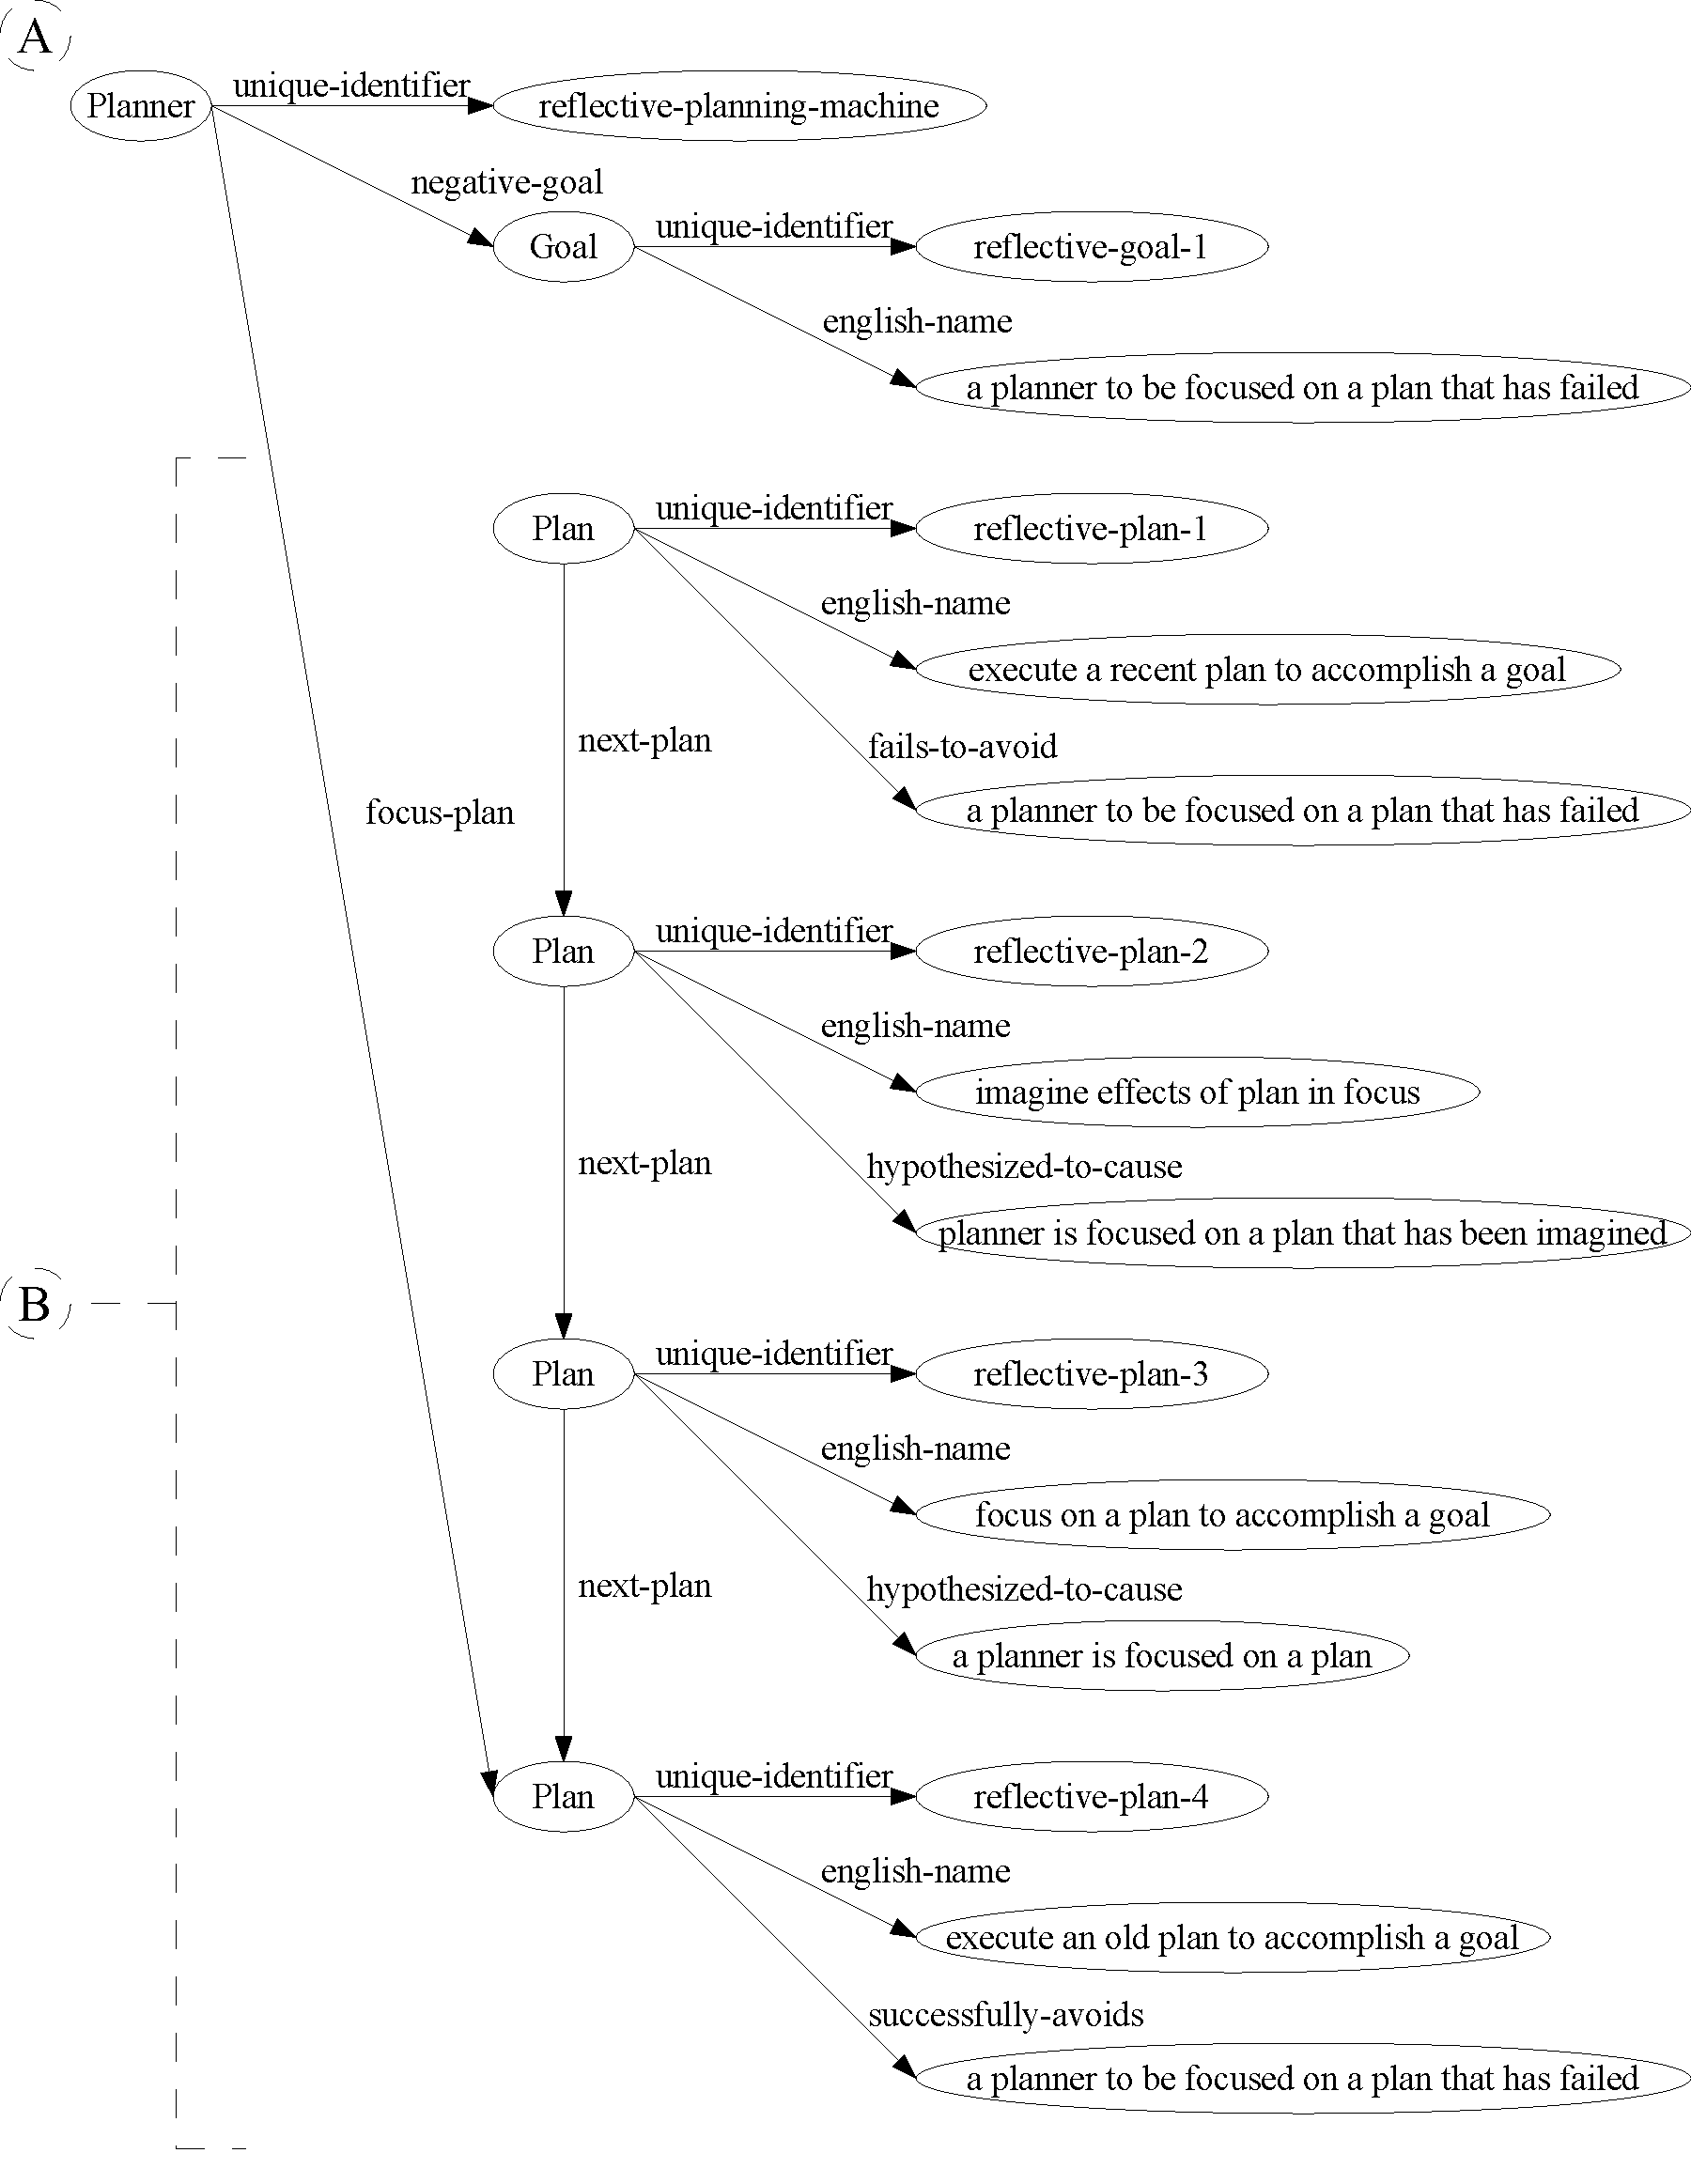
\includegraphics[height=5in]{gfx/reflective_plan_knowledge_base_graph-handdrawn}
%% \hspace{0cm}\parbox{15cm}{\caption[A simplified graph representation
%%     of the reflective plan knowledge base.]{A simplified graph
%%     representation of the reflective plan knowledge base, where
%%     frame-based objects become interconnected collections of
%%     elliptical node labels and rectangular edge labels.  The
%%     reflective planner node is at the top of the graph.  This planner
%%     is ``focused'' on a linked list of reflective plan objects.  The
%%     planner has one negative goal: ``{\tt{a planner to be focusing on
%%         a plan that has failed}}.''  The causal effects of the first
%%     plan have been imagined and are listed as properties of the plan
%%     object.  The execution node structure of the reflective
%%     imagination process are not shown for visual simplicity.  Note
%%     that the partial states in the reflective plan knowledge base are
%%     about the deliberative plan knowledge
%%     base.}\label{figure:reflective_plan_knowledge_base_graph}}
%% \end{sidewaysfigure}
Although the reflective layer of the SALS cognitive architecture is
superficially similar to the deliberative layer, the type of knowledge
that the reflective layer reasons about is categorically different.
While the deliberative layer plans toward relatively simple physical
goals, such as ``{\tt{a cube to be on a pyramid}},'' the partial
states in the reflective layer are the much more complex partial
states of the deliberative layer below, such as ``{\tt{a planner to be
    focusing on a plan that is hypothesized to cause a cube to be on a
    pyramid}}.''  Because of the categorically different types of
knowledge in different planning layers, each planning layer has a
separate communication path for being told natural language plans.  In
general, natural language plans in the deliberative layer are about
controlling the physical robot arm, while natural language plans in
the reflective layer are about controlling the deliberative planner.

\section{The Super-Reflective Layer}
\label{section:the_super_reflective_layer}

The super-reflective layer is the third planning layer in the SALS
cognitive architecture, after the deliberative and reflective layers.
The learning examples in this dissertation are focused on two layers
of learning: (1) in the deliberative layer about the physical effects
of physical actions, and (2) in the reflective layer about the
deliberative effects of deliberative actions.  To simplify the
logistics of implementing the reflective planning process in the SALS
AI, a super-reflective planning layer is included that contains
natural language plans that when executed become the reflective
planning process.  The super-reflective plans are very similar to
reflective plans because both of these layers control planning layers
below: the reflective layer controls the deliberative planning layer,
while the super-reflective layer controls the reflective planning
layer.  For example, in the story presented in
{\mbox{\autoref{chapter:introduction}}}, the super-reflective layer is
initially executing a natural language plan to ``{\tt{execute}}
{\tt{a}} {\tt{recent}} {\tt{reflective}} {\tt{plan}} {\tt{to}}
{\tt{avoid}} {\tt{all}} {\tt{negative}} {\tt{reflective}}
{\tt{goals}}.''  An analogous plan exists in the reflective layer for
finding a deliberative plan that avoids all negative deliberative
goals, partial states of the physical knowledge base.  This type of
plan search can be used in general for any reflective planning layer
that is controlling a planning layer below.  The negative reflective
goal that is being avoided in the example story is for ``{\tt{a}}
{\tt{deliberative}} {\tt{planner}} {\tt{to}} {\tt{be}} {\tt{focused}}
{\tt{on}} {\tt{a}} {\tt{plan}} {\tt{that}} {\tt{has}} {\tt{failed}}.''
In this way, the relationship between the super-reflective layer and
the reflective layer is analogous to the relationship between the
reflective layer and the deliberative layer.  Although the example
story does not include descriptions of super-reflective learning from
experience, the super-reflective layer in the SALS AI is a completely
functioning planning layer and learning from experience is implemented
and does occur in this layer as well.

I have now completed my description of the Emotion Machine cognitive
architecture included in the SALS AI.  I have described how the bottom
four layers of the Emotion Machine theory of mind have been
implemented in terms of the example story presented in
{\mbox{\autoref{chapter:introduction}}}.  These four layers of the
Emotion Machine that have been described are:
\begin{packed_enumerate}
\item{\emph{Built-In Reactive Layer}}
\item{\emph{Learned Reactive Layer}}
\item{\emph{Deliberative Layer}}
\item{\emph{Reflective Layer}}
\end{packed_enumerate}
I have also described a fifth layer that has been implemented in the
SALS AI: the {\emph{Super-Reflective Layer}}.  I see additions of
super-reflective layers as a means to implementing the
{\emph{Self-Reflective Layer}} and the {\emph{Self-Conscious Layer}}
that exist as layers five and six of the Emotion Machine theory of
mind, which I will describe briefly as future research in
{\mbox{\autoref{chapter:future}}},
{\mbox{\autoref{section:self_reflective_thinking}}} and
{\mbox{\autoref{section:self_conscious_thinking}}}.  In the next three
chapters I will describe the remaining three contributions of this
thesis:
\begin{packed_itemize}
\item{{\mbox{Chapter~\ref{chapter:learning_from_being_told}}}: Learning from Being Told Natural Language Plans}
\item{{\mbox{Chapter~\ref{chapter:learning_asynchronously_from_experience}}}: Learning Asynchronously from Experience}
\item{{\mbox{Chapter~\ref{chapter:virtual_machine_and_programming_language}}}: Virtual Machine and Programming Language}
\end{packed_itemize}
